\documentclass[12pt]{article}

\usepackage[margin=1in]{geometry}
\usepackage{amsmath,amssymb,amsthm}
\usepackage[T1]{fontenc}
\usepackage{microtype}
\usepackage{setspace}
\usepackage{parskip}
\usepackage[colorlinks=true,linkcolor=black,citecolor=black,urlcolor=black]{hyperref}
\usepackage{natbib}
\usepackage{titlesec}
\usepackage{mathpazo}
\usepackage{booktabs}
\usepackage{longtable}
\usepackage{array}
\usepackage{enumitem}
\usepackage{tikz}
\usetikzlibrary{arrows.meta,positioning,calc,decorations.pathmorphing,shapes.geometric}

\onehalfspacing

\titleformat{\section}{\large\bfseries}{\thesection.}{0.5em}{}
\titleformat{\subsection}{\normalsize\bfseries}{\thesubsection.}{0.5em}{}

\newtheorem{definition}{Definition}
\newtheorem{theorem}{Theorem}
\newtheorem{proposition}{Proposition}
\newtheorem{corollary}{Corollary}
\newtheorem{remark}{Remark}

\newcommand{\Ecal}{\mathcal{E}}
\newcommand{\Xcal}{\mathcal{X}}
\newcommand{\Mcal}{\mathcal{M}}
\newcommand{\Acal}{\mathcal{A}}
\newcommand{\Gcal}{\mathcal{G}}
\newcommand{\Lcal}{\mathcal{L}}
\newcommand{\Tcal}{\mathcal{T}}
\newcommand{\vol}{\operatorname{Vol}}
\newcommand{\E}{\mathbb{E}}
\newcommand{\R}{\mathbb{R}}
\newcommand{\kref}{\kappa(B_{\mathrm{ref}})}
\newcommand{\ktau}{\kappa(B(\tau))}

\title{\textbf{Proxy Permanence Failure}\\[0.4em]
\large Carbon Governance, Biodiversity, and the Collapse of Admissibility\\
Under Nonstationary Constraint Fields\\[0.6em]
\normalsize A Theoretical Analysis via the RSVP--TARTAN--CLIO Framework}

\author{Flyxion\\
\small Independent Researcher}

\date{May 26, 2026}

\begin{document}

\maketitle

\begin{abstract}
Three recent empirical studies expose structurally distinct failure modes in nature-based
climate solution governance, each corresponding to a different mechanism by which a
low-dimensional accounting projection loses causal adequacy as the underlying ecological
field departs from its calibration geometry. \citet{Wu2026} demonstrate that the California
Air Resources Board (CARB) buffer pool for forest carbon offsets is undersized by an
average factor of~6.3, because disturbance-risk models assume stationary ecological
conditions while wildfire, drought, and insect-outbreak probabilities accelerate under
climate forcing. \citet{Weiskopf2024} demonstrate that biodiversity loss could cause
additional global terrestrial carbon losses of 7--146~PgC through mechanisms invisible to
Earth System Models that reduce vegetation to a small number of plant functional types.
\citet{Watanabe2026} demonstrate that recalcitrant dissolved organic carbon (RDOC) from
marine macrophytes---constituting 14--25\% of released DOC over 100-year timescales---
persists through progressive transformation accessibility contraction rather than chemical
inertness, a mechanism absent from blue carbon accounting frameworks. We formalize all
three as instances of \emph{proxy permanence failure}: the progressive decoupling of a
symbolic accounting projection $\pi:\Xcal\to\Mcal$ from its causal ecological substrate as
external forcing or internal reorganization drives the trajectory space $\Xcal$ outside the
admissibility geometry in which $\Mcal$ was calibrated. The forest ecosystem is represented
as an RSVP field triple $\Ecal(t)=(\Phi,\mathbf{v},S)$ with entropy field
$S(x,t)=\log\mu(\Omega_x(t))$. Biodiversity enters as a constraint-density field $\kappa(B)$
damping entropy production. RDOC dynamics are formalized through a transformation
accessibility field $\Tcal(x,t)=\mu(\Omega^\text{transform}_x(t))$ whose contraction
follows the reactivity continuum model. A permanence functional
$\Pi[\Ecal]=\exp(-\int_0^T\Lambda\,d\tau)=\mathbb{P}(\tau>T)$ replaces binary actuarial
permanence with a first-passage survival probability. The governance system is embedded as
a dynamical operator $\Gcal(t)=(B_p,R_m,L_c,\Sigma)$ coupled to the ecological field
through an institutional memory kernel with slow decay, establishing that proxy permanence
failure is structurally a synchronization failure: $\tau_\text{institution}\gg
\tau_\text{ecology}$. We further develop a formal connection between decoupling
inequalities in Fourier restriction theory and the CLIO (Constraint-Local Inference on
Observables) framework, showing that the CARB buffer pool undercapitalization factor
of~6.3 is a measurement of the decoupling constant $D_\pi$ for the governance projection,
and that the critical exponent structure of decoupling theory corresponds precisely to the
resilience ratio phase transition $\mathcal{R}=1$ separating metastable persistence from
collapse cascade. The unified framework transforms three empirical failures into a
generative research program for constraint-indexed carbon governance.
\end{abstract}

\bigskip

\section{Introduction}

\subsection*{The Illusion of a Fungible Stock}

The claim that forests and coastal vegetation constitute stable, tradeable carbon sinks
rests on a deceptively simple ontological premise: that carbon residing in biomass or
exported as dissolved organic matter is a durable, fungible stock, comparable across sites,
times, and perturbation regimes. This premise is institutionally convenient---it permits
the construction of ledger systems, insurance mechanisms, and market instruments operating
on actuarial logic. It is also, as a growing body of empirical literature makes clear,
increasingly false.

Three recent studies sharpen this critique with unusual precision, each exposing a
different dimension of the same underlying failure. \citet{Wu2026} analyze 116 compliance
carbon offset forest projects under the CARB Cap-and-Trade Program and find that the buffer
pool is undersized by an average factor of~6.3, ranging from 2.2 to~8.0 across sensitivity
analyses. Climate change roughly triples wildfire-driven reversal probabilities over 100
years, and 41\% of currently active projects face reversal probabilities exceeding~50\%
under a moderate emissions scenario (SSP2-4.5).

\citet{Weiskopf2024} approach the problem from a complementary direction. Linking a
macroecological model of vascular plant species persistence (BILBI) with empirical
biodiversity--biomass stock relationships \citep{OConnor2017}, they estimate that
biodiversity decline alone could cause global terrestrial carbon losses of
7.4--103.1~PgC under a global sustainability scenario and 10.9--146.0~PgC under
fossil-fueled development---losses arising because ecologically impoverished systems
maintain biomass production less effectively under given abiotic conditions, through
mechanisms that Earth System Models (ESMs) reduce to a small number of plant functional
types cannot capture \citep{Ferrier2016}.

\citet{Watanabe2026} provide a third empirical result, concerning marine rather than
terrestrial carbon: dissolved organic carbon (DOC) released by macroalgae and seagrasses
across coastal Japan retains a recalcitrant fraction of 14--25\% at the 100-year timescale,
corresponding to 4--8\% of annual net primary production (NPP). This RDOC persists not
because it is chemically inert but because it has been progressively transformed into
configurations that are dynamically inaccessible to available degradation operators---a
mechanism formalized by the reactivity continuum (RC) model and confirmed by
degradation-promoting experiments that expanded the available transformation operator set
(light exposure, nutrient addition, microbial inoculation) without substantially reducing
the residual pool.

Together these three papers expose what we formalize as \emph{proxy permanence failure}:
the progressive decoupling of a symbolic accounting projection from its causal ecological
substrate, arising when the underlying field system departs from the admissibility geometry
in which the projection was calibrated. This essay develops the RSVP (Relativistic
Scalar-Vector Plenum), TARTAN, and CLIO frameworks as a unified mathematical scaffolding
for understanding all three failures as instances of the same underlying structure. The
argument proceeds through nine sections. Sections 2--3 introduce the field representation
and unified carbon-balance equation. Section 4 develops the permanence functional and
stochastic survival interpretation. Sections 5--6 analyze the disturbance-entropy and
constraint-dimensionality mechanisms. Section 7 analyzes the RDOC accessibility-contraction
mechanism and unifies the three modes. Section 8 develops the formal connection to
decoupling theory. Section 9 embeds governance as a dynamical system with institutional
memory. Section 10 develops the resilience premium as a self-correcting field operator.
Section 11 sketches the reformulated permanence criterion.

\subsection*{Claim-Status Grammar}

This paper operates simultaneously across ecology, climate science, stochastic dynamics,
marine chemistry, governance theory, harmonic analysis, and control theory. Given this
breadth, we adopt an explicit claim-status grammar. Results are marked as follows:
\textbf{[E]}~empirical result drawn directly from the cited papers; \textbf{[F]}~formal
definition or theorem within the RSVP--TARTAN--CLIO framework; \textbf{[H]}~heuristic
correspondence---a structural parallel proposed as interpretively illuminating but not
formally derivable; \textbf{[C]}~conjectural extension---a claim advanced as internally
consistent but requiring independent formal development. The decoupling-theory section
(Section~8) is primarily \textbf{[H]}: the correspondences between Fourier restriction
geometry and ecological admissibility are structural analogies, not theorem transfers.
The governance section (Section~9) mixes \textbf{[F]} and \textbf{[C]}. The resilience
premium (Section~10) is \textbf{[C]}, developed as a candidate research program.

\subsection*{Minimal Interpretation}

The RSVP--TARTAN--CLIO framework is the primary analytical lens of this paper, but
readers skeptical of field-theoretic ecological ontology can extract a set of claims
requiring no commitment to the full framework, following directly from the three
empirical papers.

\textit{(i) Governance models fail under nonstationarity.} Buffer pools calibrated to
historical disturbance frequencies are structurally inadequate when those frequencies are
accelerating. This holds regardless of what mathematical language describes the failure
\citep{Wu2026}.

\textit{(ii) Biodiversity stabilizes carbon persistence.} The empirical relationship
$\mathrm{Biomass}\propto R^b$ means that species loss produces a first-order carbon-storage
penalty. Accounting systems that omit biodiversity as a state variable systematically
underestimate future losses \citep{Weiskopf2024}.

\textit{(iii) Permanence should be trajectory-based rather than binary.} A credit that
is ``not yet reversed'' is not the same as one that is unlikely to be reversed. The
permanence functional $\Pi[\Ecal]=\mathbb{P}(\tau>T)$ is a survival probability that any
stochastic model of forest dynamics can estimate, independently of the RSVP interpretation.

\textit{(iv) Governance lag creates synchronization failure.} When institutional update
periods substantially exceed ecological transition timescales, the governance system
applies corrections calibrated to a past state of the ecosystem. Slow governance operating
on fast-changing ecosystems generates systematic underestimation of current risk.

\textit{(v) RDOC persistence is operationally, not chemically, defined.} Recalcitrance
reflects the available transformation operator landscape. The fraction of DOC export
creditable as long-term storage depends on degradation dynamics that vary by species
composition and environmental context in ways current blue carbon frameworks do not
represent \citep{Watanabe2026}.

These five claims are empirically grounded, policy-relevant, and accessible to readers
who prefer to treat the subsequent formalism as optional interpretive scaffolding.

\section{RSVP Field Representation: Foundations and Entropy Definition}

\subsection{The Field Triple}

We represent a carbon-bearing ecosystem as an RSVP field triple
\begin{equation}
\Ecal(t) = \bigl(\Phi(x,t),\;\mathbf{v}(x,t),\;S(x,t)\bigr),
\end{equation}
where $\Phi$ is stored carbon and biomass density, $\mathbf{v}$ is material-ecological flow
(nutrient cycling, trophic flux, hydrological transport, disturbance propagation, DOC
export), and $S$ is the configurational entropy field. Carbon accounting systems treat
ecosystems as passive scalar reservoirs $C(x,t)$, discarding $\mathbf{v}$ and $S$ entirely.
The three empirical papers collectively demonstrate that the discarded variables govern
whether $\Phi$ persists.

\subsection{Measure-Theoretic Definition of the Entropy Field}

We define
\begin{equation}
\label{eq:entropy-def}
S(x,t) = \log\,\mu\!\bigl(\Omega_x(t)\bigr),
\end{equation}
where $\Omega_x(t)$ is the set of dynamically accessible future trajectories of the
ecosystem initiated from state $x$ at time $t$, and $\mu$ is a reference measure on the
trajectory space $\Xcal$. $S(x,t)$ measures the logarithmic volume of accessible
ecological futures: large when many trajectories remain open (high phase-space elasticity),
small when the system is constrained to a narrow set of paths (approaching organized
stability or deterministic collapse).

Throughout this paper we maintain a strict notational distinction: $S(x,t)=\log\mu(\Omega_x(t))$
denotes \emph{global ecological trajectory accessibility}---the log-volume of dynamically
accessible futures for the entire field state at $x$---while $\Tcal(x,t)=\mu(\Omega_x^\text{transform}(t))$,
introduced in Section~7, denotes \emph{local transformation-operator accessibility}---the
measure of the set of chemical and microbial transformation operators available to the
dissolved organic carbon pool at $(x,t)$. Both are instances of the same geometric
construction applied to different phase spaces, but they operate on structurally distinct
trajectory spaces and should not be conflated. $S$ governs ecological resilience;
$\Tcal$ governs carbon recalcitrance. A complete notation table is provided in
Appendix~\ref{app:notation}.

\subsection{Concrete Realization of the Trajectory Measure}

The measure $\mu$ in definition~\eqref{eq:entropy-def} is left abstract for generality,
but one canonical realization connects the framework to path-integral methods in
stochastic ecology. Given the SDE dynamics~\eqref{eq:sde} with rate function $I[\gamma]$
encoding the action cost of trajectory $\gamma$, define
\begin{equation}
\label{eq:path-measure}
\mu(\Omega_x(t)) = \int_{\Omega_x(t)} e^{-I[\gamma]}\,\mathcal{D}\gamma,
\end{equation}
where $\mathcal{D}\gamma$ is a reference path measure and the integral runs over
trajectories initiating from state $x$ at time $t$. High $S$ corresponds to a broad,
high-weight ensemble of recovery trajectories; low $S$ corresponds to a narrow,
low-probability corridor. This realization is not assumed throughout the paper---the
theorems hold for any reference measure satisfying standard regularity conditions---but
it grounds the entropy field in familiar probability-weighted path counting.

\subsection{Why Static State Variables Fail Under Nonstationarity}

Traditional carbon accounting assumes that the future state distribution of an ecosystem
can be represented as perturbations around a stationary baseline, making scalar state
variables---biomass stock, mean sequestration rate---sufficient summaries for actuarial
modeling. Under accelerating climate forcing this assumption fails. The probability
distribution over future ecosystem states changes through time, and the relevant object
is no longer a static state variable but the geometry of accessible trajectories. Two
forests with identical present biomass may occupy radically different regions of
trajectory space: one embedded in a broad recovery manifold, another near a narrow
collapse boundary.

The shift from stock ontology to trajectory ontology is therefore not philosophical
ornamentation but a consequence of nonstationary stochastic dynamics. Scalar accounting
appears sufficient precisely when omitted dimensions contribute only perturbatively to
system dynamics---when the ecology is operating within the near-linear, near-stationary
regime for which the projection was calibrated. The present framework argues that this
perturbative regime is progressively collapsing under climate forcing, activating the
dimensions the projection discards.

\subsection{Epistemic Compression versus Causal Compression}

Not all dimensional reduction constitutes projection failure. The relevant distinction
is between \emph{epistemic compression}---which removes variables whose omission does
not substantially alter the system's persistence geometry over the timescale of
interest---and \emph{causal compression}, which removes variables that govern
admissibility structure, recovery dynamics, synchronization thresholds, or attractor
transitions. Under causal compression, the projection remains algebraically coherent
while losing dynamical fidelity.

The central claim of this paper is that current carbon governance systems apply causal
compression. Biodiversity structure, disturbance synchronization, and transformation
accessibility are omitted despite governing whether persistence trajectories remain
admissible. The framework does not object to dimensional reduction per se; it objects
when the omitted dimensions are precisely those governing long-term persistence.

\subsection{Why Geometric Rather than Equilibrium Formalism}

Conventional carbon governance models are primarily equilibrium-based: they assume
systems fluctuate around approximately stationary statistical distributions, making
scalar state variables adequate summaries. The present framework adopts a geometric
perspective because the relevant problem is not small fluctuation around equilibrium
but deformation of the accessible trajectory space itself. Climate forcing alters
$\Omega_x(t)$, $\vol(\Acal)$, $\dim_C$, and $\mathcal{D}(t)$---the topology and
geometry of admissible futures evolve through time. Under such conditions, equilibrium
statistics become insufficient because the future trajectory space is no longer sampled
from the same distribution as the past, making historical calibration a form of
structural ignorance rather than merely imprecise parameter estimation.

\subsection{Ecological Heterogeneity as Curvature}

The repeated use of geometric language throughout this paper is not merely metaphorical.
Curvature, in the present context, refers to the degree to which local perturbations
change the admissible trajectory structure of neighboring regions. Flat systems permit
near-independent local decomposition: perturbations remain localized and additive
approximations remain stable. Curved systems exhibit strong local-to-global coupling:
small perturbations alter recovery geometry nonlinearly across scales.

Biodiversity gradients, hydrological feedbacks, fire-weather synchronization, and
microbial accessibility dynamics all introduce curvature into the ecological field.
The failure of flat-rate governance projections is therefore structurally analogous to
the failure of linear approximations on highly curved manifolds---not because ecology
is a manifold in the differential-geometric sense, but because the same underlying
logic applies: projections calibrated to local linear behavior lose fidelity when
the system's interaction geometry is nonlinear.

\subsection{The Unified Carbon-Balance Equation}

A minimal carbon-balance equation integrating all three papers' results is
\begin{equation}
\label{eq:carbon-balance}
\frac{\partial\Phi}{\partial t}
= -\nabla\cdot(\Phi\,\mathbf{v})
+ G(B,\Phi,\theta)
- D(\theta,t)\,\Phi
- \mu(B,\theta)\,\Phi
- \mathcal{R}(\Tcal,S,\mathbf{v})\,\Phi_\text{DOC},
\end{equation}
where $B$ is biodiversity, $\theta$ is climate and land-use forcing, $G$ is growth and
sequestration, $D(\theta,t)$ is acute disturbance loss, $\mu(B,\theta)$ is chronic
biodiversity-mediated degradation, and $\mathcal{R}(\Tcal,S,\mathbf{v})\Phi_\text{DOC}$
is accessibility-weighted degradation of dissolved organic carbon through transformation
operator depletion. The Wu et al.\ paper primarily concerns $D(\theta,t)$; Weiskopf et al.\
concern the $B$-dependence of $G$ and $\mu$; Watanabe et al.\ concern $\mathcal{R}(\Tcal)$.

\subsection{The Projection and Admissibility}

\begin{definition}[Admissibility manifold]
The \emph{admissibility manifold} $\Acal(t)\subseteq\Xcal$ is the set of ecological
trajectories compatible with the governance assumptions embedded in the projection
$\Mcal$ at $t$: the disturbance frequency distributions, biomass persistence assumptions,
DOC recalcitrance fractions, and stationarity conditions on which the protocol's
actuarial calculations are based.
\end{definition}

The admissibility volume is $\vol(\Acal)=\int_{\Acal}d\mu(\gamma)$, using the same
reference measure as~\eqref{eq:entropy-def}.

\begin{definition}[Proxy permanence failure]
\emph{Proxy permanence failure} occurs when $\Acal(t)$, as embedded in $\Mcal$, becomes
progressively decoupled from the true trajectory space $\Xcal$ as external forcing or
internal reorganization reshapes the underlying dynamics in ways not reflected in $\Mcal$.
The projection retains its formal properties while its causal content degrades: symbolic
permanence is maintained while physical permanence capacity erodes.
\end{definition}

\section{Unified Mathematical Treatment}

\subsection{Biodiversity-Mediated Carbon Loss}

The empirical biodiversity--biomass relationship \citep{OConnor2017}:
$\text{Biomass} = aR^b$ with $b=0.26$ (95\% CI: $0.16$--$0.37$). In proportional form,
$p_{\text{biomass}}=p_R^b$, giving
\begin{equation}
\label{eq:bio-loss}
\Delta C_{\text{bio}} = C_0\bigl(1-p_R^b\bigr) \approx C_0 b\,\varepsilon + O(\varepsilon^2),
\end{equation}
for fractional species loss $\varepsilon \ll 1$. Biodiversity loss creates a first-order
carbon-storage penalty invisible to any model that omits $B$ from its state representation.

\subsection{Nonstationary Reversal Probability}

Under stationary historical rates, $P_i^{100}=1-(1-p_i)^{100}$. Under climate forcing:
\begin{equation}
\label{eq:reversal-prob}
P_i^{100}(\theta) = 1-\prod_{t=1}^{100}\bigl(1-p_i^{\text{hist}}\,r_i(t,\theta)\bigr),
\end{equation}
where $r_i(t,\theta)$ encodes projected climate-driven frequency changes from six CMIP6
models. For wildfire under SSP2-4.5, $r_\text{fire} \approx 3.3$ by end of century.

\subsection{RDOC Accessibility Contraction}

The RC model \citep{Watanabe2026}:
\begin{equation}
\label{eq:rc-model}
\text{DOC}_{Mt} = \text{DOC}_{M0}\left(\frac{\alpha}{\alpha+t}\right)^\nu,
\quad k(t) = \frac{\nu}{\alpha+t} \to 0,
\end{equation}
with $\alpha$ the average lifetime of reactive compounds and $\nu\in(0,1]$ the reactivity
distribution shape parameter. The RDOC fraction persisting at horizon $T$ is
\begin{equation}
\label{eq:rdoc-fraction}
\Pi_\text{RDOC} = \left(\frac{\alpha}{\alpha+T}\right)^\nu,
\end{equation}
with $T=100$ years giving mean values of 25\% for seagrasses and 14\% for macroalgae.

\subsection{Combined Expected Carbon Loss}

Integrating all three effects:
\begin{equation}
\label{eq:combined}
\E[\Delta C]
= \underbrace{C_0\bigl(1-p_R^b\bigr)}_{\text{biodiversity loss}}
+ \underbrace{C_0\,p_R^b\!\left[1-\prod_{t=1}^{100}(1-p_D(t))\right]\sigma}_{\text{disturbance reversal}}
+ \underbrace{\text{DOC}_{M0}\bigl(1-\Pi_\text{RDOC}\bigr)}_{\text{accessibility contraction}},
\end{equation}
where $p_D(t)$ is combined disturbance probability and $\sigma$ is disturbance severity.
The three terms correspond to the three empirical papers and the three failure modes.
Current governance instruments address only a fraction of the second term, calibrated to
stationary $p_D$ with $\sigma$ and $p_R$ held constant.

\subsection{The ESM Projection Gap}

ESMs apply $\pi_\text{ESM}:\Xcal\to\R^k$ with $k\leq 15$ plant functional types and
$\dim(\Xcal)\gg k$. Under stable historical conditions, discarded dimensions have
negligible perturbative contribution. Under climate forcing, biodiversity collapse
activates the omitted dimensions: species-level responses, functional complementarity
under novel disturbance regimes, and within-PFT compositional turnover become causally
dominant. The projection error is systematic omission of the variables governing whether
the low-dimensional dynamics remain valid.

\section{The Permanence Functional and Survival Interpretation}

\subsection{Definition and Destabilization Rate}

\begin{equation}
\label{eq:permanence-functional}
\Pi[\Ecal]
= \exp\!\left(-\int_0^T \Lambda(\tau)\,d\tau\right),
\end{equation}
with
\begin{equation}
\label{eq:lambda}
\Lambda(\tau)
= \lambda_1\,\mathcal{D}(\tau,\theta)
+ \lambda_2\,\frac{\kref-\ktau}{\kref}
+ \lambda_3\,\frac{dS}{dt}\bigg|_\tau
+ \lambda_4\,\frac{d\ln\Tcal}{dt}\bigg|_\tau,
\end{equation}
where the four terms represent: disturbance intensity; constraint erosion (biodiversity
loss relative to reference); entropy acceleration; and transformation accessibility
contraction rate. The fourth term is new relative to the previous draft, integrating the
Watanabe et al.\ RDOC mechanism. Effective credited carbon: $C_\text{eff}=\Pi[\Ecal]\cdot
C_0$.

\subsection{Stochastic Dynamics and First-Passage Survival}

\begin{equation}
\label{eq:sde}
d\Phi_t = f(\Phi_t, B_t, \theta_t, \Tcal_t)\,dt + \sigma(\Phi_t,\theta_t)\,dW_t,
\end{equation}
with $\tau = \inf\{t\geq 0:\Phi_t<\Phi_{\min}\}$ the first exit time from the
crediting threshold. Then $\Pi[\Ecal]=\mathbb{P}(\tau>T)$: the permanence functional is
the first-passage survival probability over the accounting horizon $T=100$ years.

\begin{proposition}[Buffer pool as permanence functional discrepancy]
The CARB buffer contribution $B_i$ is intended to approximate $C_0(1-\Pi[\Ecal_i])$.
Current protocol sets $\Pi$ to a value calibrated at $\theta_0$ with $B=B_\text{ref}$,
$\Lambda=\mathrm{const}$, and $\Tcal$ unconstrained. As $\theta$ increases, $B$ decreases,
and $\Tcal$ contracts, $\Pi[\Ecal_i]$ falls below its calibration value without update to
$B_i$, generating the undercapitalization documented by \citet{Wu2026}.
\end{proposition}

\section{Nonstationary Admissibility Collapse}

\subsection{Disturbance Entropy and Reversal Topology}

Climate change restructures the stochastic geometry of $\Xcal$: the entropy-accessible
disturbance manifold $\mathcal{D}(t)$ grows, and trajectories keeping a forest within
$\Acal$ become a shrinking fraction of all dynamically probable paths.

\begin{proposition}[Actuarial collapse under accelerating disturbance entropy]
Let $\mathcal{D}(t)$ denote the accessible disturbance manifold volume at time $t$,
and let $B_i(t_0)$ be a buffer pool calibrated under stationarity at $t_0$. If
$\mathcal{D}(t)>\mathcal{D}(t_0)$ for $t>t_0$, then $B_i(t_0)$ systematically understates
required buffer for all $t>t_0$, with gap growing monotonically with disturbance-entropy
increase rate. No within-protocol mechanism corrects this gap under maintained stationarity.
\end{proposition}

\subsection{The Resilience Ratio and Phase Transition}

\begin{equation}
\label{eq:resilience-ratio}
\mathcal{R}(t)
= \frac{\beta\,\kappa(B(t))}{\alpha\,\dot{\mathcal{D}}(t)}.
\end{equation}
Three regimes: $\mathcal{R}>1$ (metastable persistence), $\mathcal{R}=1$ (critical slowing
down), $\mathcal{R}<1$ (collapse cascade). As climate forcing increases $\dot{\mathcal{D}}$
and biodiversity loss decreases $\kappa(B)$, $\mathcal{R}$ decreases from above to below
unity. The transition at $\mathcal{R}=1$ is the phase boundary between meaningful insurance
and actuarial collapse. That 41\% of enrolled projects already show reversal probabilities
exceeding 50\% under SSP2-4.5 suggests a significant fraction has crossed below
$\mathcal{R}=1$ or operates near the critical boundary.

\subsection{Spatial Heterogeneity and Projection Homogenization}

The flat-rate buffer contribution treats all enrolled forests as exchangeable risks.
Combined disturbance probabilities under SSP2-4.5 reach 46--68\% in the Intermountain
West and California while Great Lakes forests face primarily drought risk at lower
probabilities. The projection discards spatial gradient information that is causally
constitutive of the risk distribution, concentrating unmodeled risk precisely where
accelerating disturbance entropy is most intense.

\section{Constraint Dimensionality Reduction and Biodiversity}

\subsection{Biodiversity as Distributed Constraint Architecture}

ESMs reduce global vegetation to $k$ plant functional types via $\pi_\text{ESM}:\Xcal\to\R^k$,
eliminating the within-category diversity that constitutes constraint architecture
\citep{Juarrero1999}. The mechanisms underlying $\text{Biomass}\propto R^b$---niche
partitioning \citep{Tilman1997,Loreau2001}, functional complementarity \citep{Hooper2005},
species richness effects \citep{Cardinale2012}, functional redundancy \citep{Reich2012,Duffy2017}---
are constraint-network phenomena: partially overlapping, non-identical channels through
which incoming perturbations are absorbed and redistributed.

\begin{definition}[Constraint dimensionality]
The \emph{constraint dimensionality} $\dim_C(\Xcal,t)$ is the effective dimensionality
of the constraint network stabilizing the ecosystem's organized state: the number of
partially independent channels through which disturbances can be absorbed or compensated
without triggering irreversible negentropic collapse.
\end{definition}

\subsection{Biodiversity as Constraint-Density Field and Entropy Damping}

\begin{equation}
\label{eq:entropy-evo}
\frac{\partial S}{\partial t}
= \alpha\,D(\theta,t)
- \beta\,\kappa(B)
+ \gamma\,|\nabla\Phi|^2
+ \eta.
\end{equation}
Since $\kappa'(B)>0$: $B\downarrow \Rightarrow \kappa(B)\downarrow \Rightarrow
\partial S/\partial t\uparrow \Rightarrow$ enlarged accessible collapse space.

\subsection{The Admissibility Volume Theorem}

\begin{theorem}[Dual control of admissibility volume]
Under dynamics~\eqref{eq:carbon-balance} and~\eqref{eq:entropy-evo}, with
$\Acal(t)=\{\gamma:\Phi(\gamma(\tau))\geq\Phi_{\min},\;S(\gamma(\tau))\leq S_{\max}\}$:
\begin{equation}
\frac{\partial\,\vol(\Acal)}{\partial B}>0,
\qquad
\frac{\partial\,\vol(\Acal)}{\partial D}<0.
\end{equation}
Biodiversity expands the volume of admissible resilience trajectories; climate-driven
disturbance contracts it. The effects compound multiplicatively.
\end{theorem}

\begin{proof}[Proof sketch]
Higher $B$ increases $\kappa(B)$, reducing $\partial S/\partial t$, extending the set
of $\gamma$ satisfying $S(\gamma(\tau))\leq S_{\max}$, increasing $\vol(\Acal)$.
Higher $D(\theta,t)$ simultaneously increases $\partial S/\partial t$ and reduces $\Phi$,
contracting both constraints and decreasing $\vol(\Acal)$. Multiplicative coupling
follows from the dependence of disturbance loss on $\Phi$ which is itself diminished by
$\mu(B,\theta)$.
\end{proof}

\begin{corollary}[Formal projection failure]
Two ecosystems $\Ecal_1,\Ecal_2$ may satisfy $\pi(\Ecal_1)=\pi(\Ecal_2)$ while having
$P_\text{reversal}(\Ecal_1)\neq P_\text{reversal}(\Ecal_2)$,
$\vol(\Acal_1)\neq\vol(\Acal_2)$, and
$\Pi[\Ecal_1]\neq\Pi[\Ecal_2]$.
\end{corollary}

\subsection{CLIO Distributed Inference}

A biodiverse ecosystem performs distributed inference across environmental fluctuations:
different species encode partially overlapping response strategies to drought, heat,
pathogens, and disturbance. Species are constraint operators---local encoders of adaptive
response collectively constituting the ecosystem's inferential capacity. Biodiversity loss
reduces epistemic resolution: fewer constraint channels through which perturbation can be
absorbed into recoverable trajectories. This interpretation aligns with the
Weiskopf et al.\ emphasis on complementarity and the finding that diversity-productivity
relationships strengthen over time \citep{Reich2012,Wang2016}.

\section{Recalcitrance as Trajectory Exclusion: A Third Mode}

\subsection{The RDOC Result and Its Ontological Significance}

\citet{Watanabe2026} quantify DOC release rates and recalcitrance across more than twenty
macroalgal and six seagrass species across coastal Japan, using the RC
model~\eqref{eq:rc-model} fitted to 300-day degradation experiments. Mean recalcitrant
fractions over 100 years are 25\% (95\% CrI: 17--34\%) for seagrasses and 14\%
(95\% CrI: 11--16\%) for macroalgae, corresponding to approximately 8\% and 4\% of
annual NPP respectively. RDOC export constitutes a carbon storage pathway comparable in
magnitude to particulate organic carbon burial---yet virtually absent from blue carbon
accounting frameworks.

Standard carbon accounting treats persistence as binary: carbon is either present in an
identified reservoir or has been released. The RDOC result demonstrates that persistence
is geometric: it reflects the progressive contraction of the transformation manifold as
reactive compounds are depleted and the remaining pool becomes increasingly enriched in
low-reactivity configurations. Carbon is not stored by being locked in place; it is stored
by being progressively excluded from admissible transformation pathways.

\subsection{The Transformation Accessibility Field}

Define the \emph{transformation accessibility field}
\begin{equation}
\label{eq:accessibility}
\Tcal(x,t) = \mu\!\bigl(\Omega^\text{transform}_x(t)\bigr),
\end{equation}
where $\Omega^\text{transform}_x(t)$ is the set of transformation operators (microbial,
photochemical, abiotic) dynamically accessible to the DOC pool at $(x,t)$. This is the
DOC analogue of $S(x,t)=\log\mu(\Omega_x(t))$. The RC model describes the dynamics of
$\Tcal$:
\begin{equation}
\label{eq:rdoc-dynamics}
\frac{\partial\Tcal}{\partial t} = -\mathcal{R}(\Tcal,S,\mathbf{v})\,\Tcal,
\end{equation}
where $\mathcal{R}\to 0$ as $\Tcal\to\Tcal_{\min}$: the residual accessibility of the
recalcitrant fraction. The power-law decay rate $k(t)=\nu/(\alpha+t)\to 0$ reflects
progressive contraction of $\Tcal$ as accessible reactive compounds are depleted. The
shape parameter $\nu$ controls contraction speed: $\nu\to 1$ (homogeneous pool, fast
contraction); $\nu\to 0$ (heterogeneous pool, asymptotically slow contraction).

\begin{definition}[Recalcitrance as dynamical inaccessibility]
A carbon pool is \emph{recalcitrant} at time $t$ if $\Tcal(x,t)<\Tcal_c$, where
$\Tcal_c$ is a threshold accessibility below which available transformation operators
cannot efficiently process the pool under ambient conditions. Recalcitrance is an
\emph{operational inadmissibility}---a relational property of the pool relative to the
available transformation operator landscape, not an intrinsic chemical property.
\end{definition}

This operationalizes the RSVP distinction between intrinsic impossibility and operational
inadmissibility. The degradation-promoting experiments of \citet{Watanabe2026}---in which
light exposure, nutrient enrichment, and new microbial inocula barely affected the residual
RDOC pool---confirm this interpretation: expanding the available transformation operator
set does not substantially degrade the recalcitrant fraction, because its inaccessibility
is determined by the molecular ensemble configuration, not by extrinsic limiting factors.

\subsection{FDOM Reorganization and Recursive Admissibility Contraction}

The FDOM analysis reveals that during 300-day degradation, humic-like components (C1,
C2, C3) \emph{increased} by a factor of approximately~1.2, while protein-like components
(C4) decreased by a factor of approximately~0.4. The system is not merely losing carbon;
it is reorganizing into lower-accessibility configurations. In RSVP terms: microbial
metabolism redistributes accessibility density---converting high-$\Tcal$ bioavailable
substrate into low-$\Tcal$ humic-like compounds via the microbial carbon pump. This is
\emph{recursive admissibility contraction}: the degradation process itself generates the
recalcitrant residue, in a manner that depends on both substrate chemistry and microbial
community diversity $B$.

\subsection{A Unified Three-Mode Taxonomy}

The three empirical papers identify three distinct mechanisms of proxy permanence failure:

\begin{enumerate}[leftmargin=*,label=\textbf{\arabic*.}]
\item \textbf{Disturbance entropy expansion} (Wu et al.): Accessible high-reversal
trajectory volume grows under climate forcing; the buffer pool remains calibrated to
obsolete $\mathcal{D}(t_0)$.

\item \textbf{Constraint dimensionality reduction} (Weiskopf et al.): Biodiversity
erosion removes constraint channels, contracting $\vol(\Acal)$ in dimensions invisible
to the projection.

\item \textbf{Transformation accessibility contraction} (Watanabe et al.): Progressive
depletion of reactive compounds and reorganization into humic configurations contracts
$\Tcal(x,t)$ asymptotically; the full DOC export value $\text{DOC}_{M0}$ is credited
while the physical variable governing persistence is the trajectory of $\Tcal$ over
the accounting horizon.
\end{enumerate}

All three discard from $\pi$ the dynamical variable ($\mathcal{D}$, $\kappa(B)$, or
$\Tcal$) governing whether the projected carbon value remains physically meaningful. The
RDOC mechanism has a closed-form permanence functional~\eqref{eq:rdoc-fraction}:
$\Pi_\text{RDOC}=(\alpha/(\alpha+T))^\nu$, making $C_\text{eff}=\Pi_\text{RDOC}\cdot
\text{DOC}_{M0}$ the blue-carbon analogue of the forest permanence functional~\eqref{eq:permanence-functional}.

\subsection{RC Model as RSVP Field Dynamics}

The full coupled system integrating DOC and accessibility dynamics:
\begin{align}
\frac{\partial\Phi_\text{DOC}}{\partial t}
&= -\nabla\cdot(\Phi_\text{DOC}\,\mathbf{v})
   - \mathcal{R}(\Tcal,S,\mathbf{v})\,\Phi_\text{DOC},\\[4pt]
\frac{\partial\Tcal}{\partial t}
&= -\mathcal{R}(\Tcal,S,\mathbf{v})\,\Tcal
   + \mathcal{F}_\text{MCP}(\Phi_\text{DOC},B),
\end{align}
where $\mathcal{F}_\text{MCP}(\Phi_\text{DOC},B)$ is the microbial carbon pump term:
production of low-$\Tcal$ humic-like compounds from high-$\Tcal$ bioavailable substrate,
dependent on microbial community diversity $B$. This connects the RDOC mechanism to
the biodiversity constraint-density field: $\kappa(B)$ governs both ecosystem resilience
against disturbance and the efficiency of the microbial carbon pump in generating RDOC.

\section{Decoupling Theory and the CLIO Inference Geometry}

\subsection{Structural Correspondence: A Methodological Note}

The correspondences developed in this section are \textbf{[H]}~heuristic: the Bourgain--Demeter
theorem and its extensions are results in harmonic analysis and do not, by themselves, imply
anything about ecological systems. What we propose is a \emph{structural analogy}---a parallel
between the mathematical architecture of decoupling inequalities and the mathematical
architecture of CLIO distributed inference---that we find illuminating and that may suggest
productive directions for formal development. Readers should interpret claims in this section
as: ``the following structural feature of decoupling theory has a counterpart in CLIO with
the following formal properties,'' not as: ``the decoupling theorem implies this property of
ecosystems.'' The wave-packet--TARTAN correspondence (Section~8.4) and the no-universal-projection
conclusion (Section~8.5) are the parts of this section we consider most robust.

\subsection{Structural Analogy versus Dynamical Identity}

The correspondences developed throughout Sections~8--9 should not be interpreted as claims of
dynamical identity between ecological systems and harmonic-analytic or machine-learning systems.
The Bourgain--Demeter theorem does not imply ecological resilience bounds; wave-packet
localization does not imply literal TARTAN tiling dynamics in forests or marine systems; and
the scale-vector preconditioning result of \citet{Wang2026} does not imply that biodiversity
literally functions as a neural normalization layer. The proposed correspondences operate at
the level of formal architecture: local-to-global reconstruction, multiscale admissibility,
coupling amplification, and curvature-sensitive projection fidelity.

The utility of these analogies is organizational rather than derivational. They provide a
shared vocabulary for understanding why low-dimensional projections fail under nonlinear
synchronization and why latent structural variables govern persistence while remaining
invisible to coarse metrics. The framework therefore advances no claim that ecological systems
obey Fourier restriction dynamics or neural optimization dynamics in any literal physical
sense.

\subsection{Correspondence Lexicon}

Table~\ref{tab:lexicon} provides a compact translation between the harmonic-analysis
terms used in this section and their ecological counterparts. Readers fluent in one domain
but not the other may find it useful to keep this table in view while reading
Sections~8.3--8.7.

\begin{table}[h]
\centering
\caption{Structural correspondence lexicon for Section~8.}
\label{tab:lexicon}
\renewcommand{\arraystretch}{1.3}
\begin{tabular}{@{}p{4.8cm}p{7.0cm}@{}}
\toprule
\textbf{Harmonic analysis} & \textbf{Ecological / governance counterpart} \\
\midrule
Frequency cap $\theta$ on the parabola
  & Disturbance regime tile (wildfire, drought, insect) \\
Wave packet (spatially + frequency localized)
  & TARTAN tile (spatially + perturbation-frequency + timescale localized) \\
$\delta$-cap partition at scale $R^{-1/2}$
  & Supersection-level disturbance partition \\
Decoupling constant $D_p(R)$
  & Projection fidelity gap $D_\pi$ (actual loss / projected coverage) \\
Small $D_p$: tiles approximately independent
  & $\mathcal{R}>1$: disturbance events approximately independent, recovery local \\
Large $D_p$: tiles synchronize
  & $\mathcal{R}<1$: disturbance events synchronize, cascade defeats local recovery \\
Critical exponent $p_c$ (balance of constructive interference and cancellation)
  & Resilience ratio threshold $\mathcal{R}=1$ (balance of constraint damping and disturbance entropy) \\
Curvature of the parabola
  & Nonlinearity of ecological interaction geometry ($\kappa(B)$, $\Gamma_{ij}$) \\
Auxiliary Schwarz function $\psi$ (norm-controlled inter-scale mediator)
  & Monitoring instrument translating fine-grained ecological state to governance-level accounting \\
Near-optimal $D_p(R)\lesssim(\log R)^c$ under curvature
  & Near-tight buffer pool achievable when projection captures ecological curvature geometry \\
No universal inequality dominating all regimes
  & No single flat-rate projection adequate across all disturbance types, biodiversity levels, and ecosystems \\
Induction on scales (stronger hypothesis propagates upward)
  & Recursive constraint propagation (higher-level coherence constrains lower-level admissibility) \\
\bottomrule
\end{tabular}
\end{table}

\subsection{The Decoupling Inequality as a Local-to-Global Bound}

The preceding sections have used CLIO as an interpretive framework: biodiversity provides
distributed local inference capacity and its loss reduces the ecosystem's epistemic
resolution. Here we give this idea a more precise mathematical grounding through a
structural connection to the decoupling inequalities of Fourier restriction theory
\citep{BourgainDemeter2015,Guth2016}.

The starting point is a family of functions $\{f_\theta\}$ supported on $\delta$-caps
$\theta$ partitioning a curved surface (the truncated parabola) at scale
$\delta=R^{-1/2}$. Each cap $\theta$ is approximately flat at its own scale: the
parabola has been decomposed into pieces each of which is locally like a rectangle of
dimensions $R^{-1/2}\times R^{-1}$. The $\ell^2$ decoupling inequality for the parabola
is
\begin{equation}
\label{eq:decoupling}
\left\|\sum_{\theta} f_\theta\right\|_{L^p(\R^n)}
\lesssim D_p(R)
\left(\sum_{\theta} \|f_\theta\|_{L^p(\R^n)}^2\right)^{1/2},
\end{equation}
with decoupling constant $D_p(R)$. The fundamental theorem \citep{BourgainDemeter2015}
establishes $D_p(R)\lesssim R^\varepsilon$ at the critical exponent $p=2(n+1)/(n-1)$;
subsequent work \citep{GuthMaldagueWang2022} sharpened this to
$D_p(R)\lesssim(\log R)^c$ for the parabola at $p=6$, nearly removing the logarithmic
loss. Inequality~\eqref{eq:decoupling} says: \emph{global complexity is bounded by local
complexity plus a coupling penalty}. Each $f_\theta$ is a local tile whose behavior at
its own scale is tractable; $D_p(R)$ measures how badly interactions between tiles
fail to remain independent when assembled into a global estimate.

This is the formal analytic structure of CLIO: distributed local constraint operators
whose independent contributions sum (in the $\ell^2$ sense) to bound global system
behavior, with a coupling penalty that grows precisely when local interactions become
coherently synchronized rather than independently canceling.

\subsection{From Discrete to Continuous: The Role of Auxiliary Functions}

One of the more illuminating moves in the passage from exponential sum estimates to
decoupling is the introduction of auxiliary Schwarz functions. The problem is that
exponential sums live on discrete point sets, while decoupling operates on continuous
frequency neighborhoods. The bridge is an auxiliary function $\psi$ that is roughly~$1$
on the relevant spatial domain, whose Fourier transform is supported in an inverse-sized
box, and whose $L^p$ norm is controlled so as to compensate the Jacobian factors from
rescaling.

The function $\psi$ does three things simultaneously: it enlarges spatial support (making
the domain large enough for the continuous framework), shrinks frequency uncertainty
(localizing each exponential sum term to a cap $\theta$ compatible with the decoupling
partition), and mediates the rescaling between discrete and continuous descriptions
without losing control of the norms. In RSVP terms $\psi$ is a \emph{projection
operator}: an object that translates between incompatible representational scales while
preserving the essential norm structure. The auxiliary function exists precisely because
the geometry of the parabola is curved enough to support such mediators; a flat surface
would not permit the same controlled localization.

The ecological analogue of $\psi$ is any intermediate-scale monitoring instrument that
aggregates fine-grained ecological state (species-level surveys, disturbance event records,
DOC degradation profiles) into a form compatible with governance-level accounting. The
key constraint in both settings is the same: the mediating instrument must be
norm-controlled---it must not amplify errors in translation---and this is possible only
when the underlying geometry (ecological or analytic) has sufficient curvature to constrain
the overlap between local tiles.

\subsection{Critical Exponents as Phase-Boundary Geometry}

The critical exponents arise from a competition that is worth stating precisely. Two types
of terms bound the $L^p$ norm of an exponential sum: constructive interference
$N^{p-2}$ (from the bump at the origin, where all terms add coherently) and
square-root cancellation $N^{p/2}$ (average behavior where phases cancel generically).
The critical exponent is where these balance:
\begin{equation}
\underbrace{N^{p-2}}_{\text{constructive interference}}
= \underbrace{N^{p/2}}_{\text{square-root cancellation}},
\end{equation}
giving $p_c=4$ in one spatial dimension and $p_c=6$ in two. At $p_c$, neither behavior
dominates; this is also where the number-theoretic counting argument is sharpest. The
full range of $L^p$ estimates then follows by interpolation from the endpoints ($p=2$,
where $L^2$ orthogonality is exact, and $p=\infty$, where one simply extracts the
maximum) and the critical exponent, which anchors the nontrivial estimate.

These are \emph{transition surfaces between dominant dynamical regimes}: structurally
analogous to the resilience ratio $\mathcal{R}=1$ of equation~\eqref{eq:resilience-ratio}.
Below $p_c$: cancellation dominates; tiles behave approximately independently; the global
bound is tight. Above $p_c$: constructive interference dominates; tiles synchronize; the
bound deteriorates. The transition at $p_c$ shares the same local-to-global transition
architecture as the ecological phase transition at $\mathcal{R}=1$: below each respective
threshold, a regime of incoherent (approximately independent) local dynamics permits stable
global reconstruction; above it, coherent amplification defeats modular bounds. In ecological
terms: below $\mathcal{R}=1$, disturbance events at different spatial tiles cancel in their
aggregate effect and the local-to-global recovery bound holds. Above $\mathcal{R}=1$,
disturbance events synchronize---regional drought priming insect outbreak priming wildfire---
and independent-tile assumptions fail, just as the $p>p_c$ regime sees coherent
amplification defeat the cancellation bound.

\subsection{Why Simple Counting Fails: The Passage to Multiscale Methods}

One of the most instructive moments in the passage to higher-dimensional decoupling is
the point where the elementary counting strategy breaks down. For the one-dimensional
quadratic exponential sum, one can count solutions to $n_1^2+n_2^2 = n_3^2+n_4^2$
exactly using number-theoretic tools, and this gives the sharp $p=4$ estimate. For the
two-dimensional Schr\"odinger equation the analogous system is $n_1^2+n_2^2+n_3^2 =
n_4^2+n_5^2+n_6^2$, the critical exponent shifts to $p=6$, and counting still works.
But for general convex sequences $\{a_n\}$ replacing $\{n^2\}$, the combinatorial
equation $a_{n_1}+a_{n_2}=a_{n_3}+a_{n_4}$ has no number-theoretic toolbox, and
even the sharp additive-energy count is an open problem.

The point is not incidental: the exactly solvable case works because the specific
algebraic structure of $n^2$ happens to make the combinatorial problem tractable. As
soon as one moves to general curvature, the algebraic structure is broken and exact
counting fails---one must move to geometric, multiscale, admissibility-based methods.
This is structurally identical to the failure of carbon accounting projections: the
flat-rate buffer pool works acceptably when forest dynamics remain within the
near-linear, near-stationary regime for which the actuarial model was calibrated
(the ``quadratic case''). As soon as climate forcing and biodiversity erosion introduce
genuine nonlinearity, the algebraic counting structure of the projection breaks down
and the model requires replacement by admissibility-based multiscale methods.

\subsection{Induction on Scales, Wave Packets, and TARTAN}

Decoupling becomes approachable through induction on scales: the full estimate at scale
$R$ is proved by induction from the estimate at scale $R^{1/2}$. The mechanism is that
choosing to prove the \emph{stronger} $\ell^2$-decoupling inequality (rather than the
weaker square-function estimate) provides a stronger inductive hypothesis at each step
of the induction---and this additional strength is precisely what closes the argument.
A weaker inductive hypothesis would not suffice; the strength feeds back into itself
productively at each scale.

The wave packets used in the proof make this multi-scale structure concrete. Each wave
packet is simultaneously spatially localized (to a tube of dimensions
$\sim R^{1/2}\times\cdots\times R$), frequency localized (Fourier support on a cap
$\theta$), and scale localized (the spatial-frequency relationship is fixed by the
parabola's curvature). All three localizations are coupled: given the frequency cap,
the spatial support is determined by the geometry, not by a free choice.

A TARTAN tile has the same three-way covariant localization: it occupies a bounded
spatial patch, responds to perturbations within a characteristic frequency band (slow
climate drift vs.\ rapid wildfire vs.\ seasonal drought), and has an adaptive response
timescale determined by $\dim_C$---its ecological complexity, not an externally imposed
parameter. The induction-on-scales proof strategy---stronger hypothesis at finer scale
propagates upward to constrain coarser-scale behavior---is structurally identical to
recursive constraint propagation in TARTAN: higher-level coherence constrains
lower-level admissibility, which recursively constrains the behavior accessible at
larger scales. In both cases, the architecture is one in which \emph{local structure
at finer scales is not merely consistent with global structure at coarser scales but
constitutive of it}.

\subsection{The Decoupling Constant as Projection Fidelity Measure}

The carbon credit projection $\pi:\Xcal\to\Mcal$ is an attempt to bound global
ecological behavior by a low-dimensional estimate. The analogue of the decoupling
constant is
\begin{equation}
\label{eq:decoupling-analogue}
D_\pi = \frac{\|\text{actual carbon loss}\|}{\|\text{projected buffer pool coverage}\|},
\end{equation}
the amplification factor by which actual carbon loss exceeds the projection's buffer
estimate. The Wu et al.\ finding $D_\pi\approx 6.3$ is a measurement of this constant:
it quantifies how far the current projection is from capturing the curvature geometry
of the actual ecological field.

The Bourgain-Demeter/Guth-Maldague-Wang results establish that $D_p(R)$ can be made
nearly optimal---$(\log R)^c$---when the projection correctly respects the curvature
of the underlying surface. The ecological analogue: if the governance projection
correctly captures the nonlinear disturbance interactions, biodiversity-mediated
constraint structure, and accessibility dynamics of the ecological field, the buffer
pool can be made nearly tight. The near-optimality result is the mathematical existence
proof that tight multi-scale governance is possible in principle. The empirical
$D_\pi\approx 6.3$ measures how far the current flat-rate projection is from achieving it.

\subsection{The Inconvenient Truth: No Universal Projection}

A recurrent observation in restriction and decoupling theory is what might be called an
inconvenient truth: square-function estimates, $\ell^2$-decoupling estimates, and
restriction estimates are not nested in a simple hierarchy---different inequalities are
sharp in different regimes, and which dominates depends on the geometry of the
specific problem. The sharp examples for the decoupling inequality are not the same
as the sharp examples for the square-function estimate; they come from different types
of configurations (wave packets rather than purely exponential-sum-type examples),
and this difference is what makes decoupling genuinely harder.

This is the analytic version of the RSVP anti-universalist stance: there is no single
globally sufficient projection of an ecological field system onto an accounting manifold.
Different coarse-grainings preserve different structures, and which is adequate depends
on the dynamical regime the system currently inhabits. The CARB flat-rate buffer pool
applies a single universal projection to an ecological field whose geometry varies by
orders of magnitude across spatial scales, climate regimes, disturbance types, biodiversity
levels, and accessibility spectra. The insistence in restriction theory on
regime-dependent, geometry-sensitive bounds---and the genuine difficulty of finding
bounds that work uniformly---shares the same structural logic as the RSVP insistence on
constraint-indexed, trajectory-sensitive permanence criteria that update as the
underlying field reorganizes.

\section{Scale Vectors and the Negligible-but-Constitutive Pattern}
\label{sec:scalevectors}

The material in this section is \textbf{[H]}~heuristic: the correspondences drawn
between LLM architecture and ecological governance are structural analogies, not formal
derivations.

A recent study by \citet{Wang2026} of scale vectors in large language model normalization
layers provides an unexpectedly precise empirical and theoretical instance of the paper's
central claim. Scale vectors $\boldsymbol{\gamma}$ in RMSNorm constitute roughly
$7.84\times 10^{-5}$ of a 1B-parameter model's total parameters. They are provably
expressively redundant in Pre-Norm architectures: for any $\boldsymbol{\gamma}$ and
linear map $W_2$, choosing $W_1 = W_2\,\mathrm{diag}(\boldsymbol{\gamma})$ absorbs the
scale vector entirely. Yet removing them substantially degrades pre-training, reducing
terminal loss by $0.015$--$0.028$ and costing $1.2$--$1.4\times$ token efficiency. The
paper's organizing question---\emph{although negligible in size and expressively
redundant, are scale vectors negligible in training?}---is structurally identical to the
proxy permanence framework's question about biodiversity: although $O(d)$ relative to
$O(d^2)$ matrix parameters, and invisible in the projection $\pi:\mathcal{X}\to\mathcal{M}$,
does it govern whether the projected quantity persists?

\subsection{The Preconditioning Mechanism as Constraint Architecture}

\citet{Wang2026} prove (Theorem~2.2) that under gradient flow, models with scale vectors
satisfy $\mathcal{L}_f(t) < \mathcal{L}_g(t)$ for all $t > 0$. The key mechanism is that
the scale vector $\gamma_j$ transforms the gradient flow into a self-amplifying preconditioned
flow. Define the effective parameter $A_f(t) := W_f(t)\,\mathrm{diag}(\boldsymbol{\gamma}(t))$.
Its $j$-th column dynamics satisfy
\begin{equation}
\dot{a}_{f,j}(t)
= \bigl(\gamma_j(t)^2 I_c + w_{f,j}(t)w_{f,j}(t)^\top\bigr)
\bigl(w^*_j - a_{f,j}(t)\bigr),
\end{equation}
inducing the state-dependent preconditioner
$P_{f,j}(t) = \gamma_j(t)^2 I_c + w_{f,j}(t)w_{f,j}(t)^\top$.
The conservation law $\gamma_j(t)^2 - \|w_{f,j}(t)\|^2 = 1$ guarantees
$\lambda_{\min}(P_{f,j}(t)) \geq \gamma_j(t)^2 \geq 1$, with strict inequality whenever
$w^*_j \neq 0$.

This is structurally the same phenomenon the proxy permanence paper formalizes as
constraint architecture: a low-dimensional structure ($O(d)$ parameters) governs the
stability of a high-dimensional dynamical system ($O(d^2)$ weights) through a
state-dependent mechanism that is invisible to any projection that reduces the system
to its output metric. In the ecological setting, $\kappa(B)$ damps entropy production
and expands the admissibility volume; in the LLM setting, $\boldsymbol{\gamma}$ shapes
the loss-descent geometry and accelerates convergence. Both mechanisms are negligible
in their respective projections ($\pi:\mathcal{X}\to\mathcal{M}$ discards $B$; parameter
count discards $\boldsymbol{\gamma}$) and both are dynamically constitutive.

The three scale-vector improvements of \citet{Wang2026}---heterogeneity, placement
reparameterization---reduce under their unified view to structured multiplicative scale
fields $W_c \mapsto W_c \odot (u_c v_c^\top)$ with $O(d_1 + d_2)$ parameters modulating
an $O(d_1 d_2)$-dimensional matrix. This is the exact scaling relationship the proxy
permanence paper identifies for $\kappa(B)$: $O(d)$ biodiversity structure governing
$O(d^2)$ ecological interaction geometry.

\subsection{Input-Norm versus Output-Norm: The Projection-Failure Corollary}

The Input-Norm / Output-Norm distinction in \citet{Wang2026} is a clean formal instance
of Corollary~1 from Section~6. Two models can satisfy $\pi(\mathcal{E}_1)=\pi(\mathcal{E}_2)$
in parameter-count space while requiring opposite treatment:

\begin{itemize}
\item Output-Norm scale vectors (not immediately followed by a linear map) directly
parameterize expressivity. Applying weight decay restricts expressivity and degrades
performance.
\item Input-Norm scale vectors (immediately followed by a linear map) add no expressivity.
Applying weight decay keeps the parameterization balanced, bounds Hessian sharpness, and
accelerates training.
\end{itemize}

Theorem~2.3 of \citet{Wang2026} proves this formally: without weight decay on
$\boldsymbol{\gamma}$, $\mathbb{E}\|\boldsymbol{\gamma}_t\|^2$ grows unbounded and
Hessian sharpness metrics $\lambda_{\max}(\nabla^2 \mathcal{L})$,
$\mathrm{Tr}(\nabla^2\mathcal{L})$, $\|\nabla^2\mathcal{L}\|_F$ diverge. With weight
decay $\mu>0$, all are uniformly bounded.

The projection that reduces both layer types to ``scale vectors'' ($\sim O(d)$ parameters,
same nominal role) discards the structural variable---position relative to subsequent
linear maps---that governs optimal training behavior. This is formally identical to
the governance projection $\pi$ discarding whether a forest's carbon is backed by
biodiverse constraint architecture (low disturbance entropy pressure, large recovery
manifold) or fragile monoculture (high $\Xi_D$, small $\vol(\mathcal{A})$), treating
both as equivalent carbon credits.

\subsection{Implication: Negligible-but-Constitutive as a General Pattern}

The structural parallel between LLM scale vectors and ecological biodiversity is worth
making explicit side-by-side before generalizing it.

\begin{table}[h]
\centering
\caption{The negligible-but-constitutive pattern across two domains.}
\label{tab:nbc}
\renewcommand{\arraystretch}{1.3}
\begin{tabular}{@{}p{3.8cm}p{4.8cm}p{4.6cm}@{}}
\toprule
\textbf{Property} & \textbf{Silicon (LLMs)} & \textbf{Carbon (Ecology)} \\
\midrule
Structural element
  & Scale vectors $\boldsymbol{\gamma}$ in RMSNorm
  & Biodiversity / species richness \\
Size in projection metric
  & $7.84\times 10^{-5}$ of 1B parameters
  & Tiny fraction of ecosystem biomass \\
Status under idealized assumptions
  & Expressively redundant (absorbs into linear maps)
  & Omitted from Earth System Models entirely \\
Dynamical role
  & Governs training convergence via self-amplifying preconditioning
  & Governs carbon persistence via constraint-density field $\kappa(B)$ \\
Consequence of removal
  & 0.015--0.028 terminal loss increase; $1.2$--$1.4\times$ token inefficiency
  & 7--146~PgC carbon loss (Weiskopf et al.\ 2024) \\
Why projection discards it
  & $O(d)$ vs $O(d^2)$ parameter count
  & Not captured by plant functional types \\
\bottomrule
\end{tabular}
\end{table}

Together, the Wang et al.\ results and the three empirical papers this essay analyzes
point toward a general pattern. Systems contain structural elements that are:

\begin{enumerate}
\item negligible in the metric by which the system is projected and governed ($7.84\times
10^{-5}$ of parameters; $O(d)$ vs $O(d^2)$; species richness vs biomass stock; DOC
accessibility vs DOC concentration),
\item expressively or informationally redundant under idealized assumptions (scale
vectors absorb into linear maps; biodiversity-productivity relationships saturate;
RDOC persistence approximates a fixed fraction),
\item dynamically constitutive: removing them or mismeasuring them substantially
degrades the system's stability, convergence, or persistence geometry.
\end{enumerate}

The proxy permanence failure identified in carbon governance is therefore not an
isolated institutional failure but an instance of a generic pattern: governance
projections calibrated to output-metric sufficiency under stationary conditions
systematically discard the constraint architecture that determines whether the projected
quantity persists when conditions change. The Wang et al.\ paper provides a case in
which this pattern is rigorously proved under controlled conditions; the three
empirical ecology papers demonstrate its consequences at Earth-system scale.

\section{Governance as Dynamical System: The Coupled Socio-Ecological Field}

\subsection{Governance State Variables}

Governance systems are not external observers; they are dynamical operators embedded in
the ecological field, feeding back through land-use decisions, market incentives, and
regulatory inertia. Define a governance state vector
\begin{equation}
\Gcal(t) = \bigl(B_p(t),\;R_m(t),\;L_c(t),\;\Sigma(t)\bigr),
\end{equation}
where $B_p$ is buffer pool capitalization, $R_m$ is market confidence, $L_c$ is land-use
compliance pressure, and $\Sigma$ is regulatory inertia. The total system is a coupled
socio-ecological field:
\begin{equation}
\Ecal_\text{total}(t) = \Ecal_\text{eco}(t)\oplus\Gcal(t).
\end{equation}

\subsection{The Institutional Memory Kernel and Synchronization Failure}

\begin{equation}
\label{eq:memory-kernel}
\Sigma(t) = \int_{-\infty}^t K(t-\tau)\,\mathcal{O}(\tau)\,d\tau,
\end{equation}
where $\mathcal{O}(\tau)$ is the observed ecological state and $K(s)=K_0 e^{-s/\tau_\text{inst}}$
decays slowly with $\tau_\text{inst}\sim$ decades. Governance decisions at $t$ are based
on $\Sigma(t)$ rather than $\mathcal{O}(t)$; when $K$ decays slowly, $\Sigma(t)$ is a
heavily time-averaged, outdated summary. This formalizes the synchronization failure:
\begin{equation}
\label{eq:sync-failure}
\tau_\text{institution} \gg \tau_\text{ecology}.
\end{equation}
Ecological attractor restructuring---climate-forced disturbance regime shifts, biodiversity
erosion, transformation accessibility contraction---occurs on timescales $\tau_\text{ecology}$
of years to decades. Protocol updates occur on timescales $\tau_\text{institution}$ of
decades to generations. This is a control system with delayed state estimation operating
on a rapidly changing nonstationary field---a configuration that guarantees instability
under generic assumptions \citep{Simon1962}.

We define the \emph{Proxy Failure Zone} as the temporal interval
$[\tau_\text{ecology},\,\tau_\text{institution}]$ during which ecological regime transitions
have already occurred but governance projections have not yet updated. Inside this zone,
the accounting manifold $\Mcal$ retains the parameters of the pre-transition regime while
the ecological trajectory space $\Xcal(t)$ has already reorganized. Carbon credits issued
inside the Proxy Failure Zone are priced against an admissibility geometry that no longer
exists. The empirical finding that 41\% of enrolled CARB projects face reversal
probabilities exceeding 50\% under a moderate emissions scenario represents the
observable signature of a market operating inside the Proxy Failure Zone.

\subsection{Goodhart Pressure and Projection Drift}

Once a projection $\pi:\Xcal\to\Mcal$ becomes economically incentivized, agents begin
optimizing the projection itself rather than the underlying ecological state. This
induces a secondary dynamical process:
\begin{equation}
\mathcal{O}(t)
\;\to\;
\pi\bigl(\mathcal{O}(t)\bigr)
\;\to\;
\mathrm{optimize}\bigl(\pi(\mathcal{O}(t))\bigr),
\end{equation}
in which $\Mcal$ becomes an attractor independent of the ecological field from which
it was originally derived. \emph{Projection drift} occurs when optimization pressure
progressively restructures the ecological system to maximize projection performance while
degrading unmeasured constraint architecture. The feedback is
\begin{equation}
\text{projection simplification}
\;\to\;
\text{optimization pressure}
\;\to\;
\text{constraint erosion}
\;\to\;
\text{projection failure}.
\end{equation}
The stronger the economic incentives attached to $\Mcal$---as in a multi-billion-dollar
compliance market---the stronger the pressure toward proxy optimization rather than
resilience preservation. This is not merely a governance design failure; it is a
dynamical amplifier of proxy permanence failure. The $D_\pi \approx 6.3$
undercapitalization factor \citep{Wu2026} may therefore partially reflect not only
stationarity assumptions but active optimization pressure that has progressively
concentrated enrolled projects in regions of high short-term credit yield and high
long-term reversal risk.

\subsection{Semantic Accessibility and Context-Conditioned Governance Memory}

The institutional memory kernel $\Sigma(t)$ introduced in equation~\eqref{eq:memory-kernel}
models governance memory as a passively filtered archive: all historical observations
enter with exponentially decaying weight, and retrieval is uniform across the historical
record. This is an idealization. In practice, institutional retrieval is not uniform;
it is conditioned on the current governance focus state.

Let $f(t)$ denote the current governance focus state---the constellation of policy
categories, accounting assumptions, and institutional priorities active at time $t$.
Define a focus-conditioned projection
\begin{equation}
\pi_f : \Xcal \to \Mcal_f,
\end{equation}
where $\Mcal_f$ is a dynamically evolving governance manifold whose geometry depends on
$f(t)$. The focus-conditioned memory accessibility field is then
\begin{equation}
\label{eq:access-field}
\Acal_f(t) = \bigl\{\gamma\in\Xcal : \rho(\gamma, f) > \epsilon\bigr\},
\end{equation}
where $\rho(\gamma, f)$ measures semantic resonance between the historical ecological
trajectory $\gamma$ and the current governance focus state, and $\epsilon$ is a
retrieval threshold. Historical records may physically exist while becoming operationally
inaccessible because the retrieval geometry $\pi_f$ no longer exposes them under current
institutional attention operators.

This extends the earlier distinction between epistemic compression and causal compression
(Section~2) into a second-order form. First-order proxy permanence failure occurs when
the governance projection discards variables governing ecological persistence. Second-order
proxy permanence failure occurs when the institutional memory system discards historical
trajectories that would have revealed the first-order failure, because those trajectories
lie outside $\Acal_f(t)$: they are physically stored but focus-inaccessible.

The result is recursively self-stabilizing: institutions that have formed strong
governance focus states around object-ontology accounting categories will tend to
retrieve historical records that confirm object-ontology adequacy, reinforcing the
projection that initially bounded retrieval. This is the semantic analogue of the
Goodhart pressure loop formalized in the preceding subsection. Just as market incentives
drive ecological restructuring toward projection performance, retrieval geometry drives
institutional memory toward focus-confirming trajectories.

Biodiversity already functions in this paper as distributed ecological inference: overlapping
species response profiles provide redundant causal channels for absorbing perturbation
and updating the system's accessible recovery manifold. Institutional memory can be
understood as a parallel distributed inference field operating over historical trajectories
rather than biological response channels. When that inference field becomes focus-locked,
it loses the same compensatory channel diversity that a species-impoverished ecosystem
loses: the capacity to respond to perturbations that fall outside the active projection
geometry.

\subsection{Constructive Reinforcement and Informational Attractor Formation}

Repeated retrieval and governance emphasis do not merely preserve records; they amplify
particular trajectory basins within the institutional memory field while suppressing
others. Institutional memory therefore behaves like a nonlinear reinforcement field
rather than a neutral archive.

Define a trajectory salience amplitude field $A_t(x)$ evolving under the reinforcement
dynamics
\begin{equation}
\label{eq:reinforcement}
A_{t+1}(x) = A_t(x) + \alpha\,\phi(x,t) - \lambda A_t(x),
\end{equation}
where $\phi(x,t)$ is retrieval or governance emphasis intensity at trajectory region $x$
at time $t$, $\alpha > 0$ is the reinforcement rate, and $\lambda > 0$ is the natural
decay rate. Equation~\eqref{eq:reinforcement} is a discrete-time analogue of the
continuous dynamics underlying the reinforcement fields already present in the paper:
disturbance amplification (Section~5), biodiversity damping via $\kappa(B)$ (Section~6),
RDOC persistence via the RC model (Section~7), and governance lag via $\Sigma(t)$
(Section~10.2).

Governance systems naturally form \emph{informational attractors}: highly reinforced
policy categories, disturbance narratives, or accounting assumptions that become
increasingly stable under recursive retrieval even when ecological conditions have changed.
The fixed points of equation~\eqref{eq:reinforcement} satisfy $A^*(x) = \alpha\phi(x)/\lambda$:
the long-run salience landscape is shaped entirely by the retrieval intensity distribution
$\phi(x)$, not by the ecological significance of the trajectories at $x$. High
administrative emphasis produces high salience independently of physical relevance.

\begin{proposition}[Informational Attractor Stability]
\label{prop:attractor}
\textbf{[C]} Under the reinforcement dynamics~\eqref{eq:reinforcement} with $\alpha,\lambda>0$,
the salience field converges to a fixed-point distribution
$A^*(x) = \alpha\phi(x)/\lambda$ independently of the initial salience distribution
$A_0(x)$. If the retrieval intensity $\phi(x,t)$ is governed by the current governance
focus state $f(t)$ rather than by ecological significance, then $A^*(x)$ may diverge
arbitrarily from the ecologically optimal salience distribution, and the informational
attractor will be maintained as a stable configuration even after the ecological
conditions that originally justified it have ceased to hold.
\end{proposition}

This proposition connects directly to the model-collapse argument of Section~15. Projection
coherence can be maintained not only because governance accounting rules remain internally
consistent, but because the informational attractor reinforces the institutional attention
patterns that prevent recognition of ecological regime transition. The attractor is
self-sealing: the more economically and institutionally consequential a governance
category, the higher $\phi(x)$ becomes, the deeper the attractor, and the harder the
retrieval geometry becomes to shift even when physical reality has moved outside its
basin.

\textbf{Relationship to Goodhart pressure.} The Goodhart pressure loop (Section~10.3)
operates through economic incentives restructuring ecological systems toward projection
performance. The informational attractor mechanism operates through retrieval dynamics
restructuring institutional memory toward focus-confirming histories. These are parallel
but distinct mechanisms, and they compound: ecological Goodhart restructuring reduces the
physical diversity of offset portfolios, while informational attractor formation
simultaneously reduces the epistemic diversity of the historical evidence base. Both
processes contract admissibility volume, one physically and one epistemically.

\subsection{Adaptive Compression and Institutional Forgetting}

Governance systems fail not only through excessive lag but also through excessive
archival rigidity: the accumulation of historical records in configurations that cannot
be reorganized as the relevant retrieval geometry changes. Rather than treating archival
persistence as inherently stabilizing, the framework distinguishes between preservative
accumulation and adaptive consolidation.

Define an effective governance entropy
\begin{equation}
\label{eq:gov-entropy}
S_G(t) = \log\mu\bigl(\Omega_G(t)\bigr),
\end{equation}
where $\Omega_G(t)$ is the accessible governance trajectory space under current
institutional constraints: the set of policy configurations, accounting adjustments, and
protocol revisions accessible to the governance system given its current focus state,
memory architecture, and institutional mandate. High $S_G$ corresponds to a governance
system capable of accessing diverse historical trajectory templates and reorganizing its
projections in response to ecological change. Low $S_G$ corresponds to an institutionally
rigid system whose accessible policy space has contracted to a narrow corridor around the
existing informational attractor.

Excessive archival accumulation without selective consolidation drives
\begin{equation}
\label{eq:gov-entropy-decay}
\frac{dS_G}{dt} < 0,
\end{equation}
because the volume of accessible governance trajectories is constrained by the
computational and administrative capacity to integrate historical evidence under a
changing retrieval geometry. A governance system that accumulates records without
reorganizing them cannot effectively deploy those records when its focus state shifts.
The archive grows while the accessible trajectory space contracts.

This reinforces the paper's central anti-static ontology with a governance-theoretic
corollary: persistence is not storage, permanence is not binary, resilience is not
accumulation, and governance failure is fundamentally geometric. The appropriate
analogue is not a larger database but a better consolidated memory field---one capable
of adaptively reorganizing its retrieval geometry as the ecological focus state changes,
selectively forgetting obsolete accounting assumptions, and exposing previously
inaccessible historical trajectories relevant to nonstationary forcing conditions.

The critical governance latency $\tau_c$ (Proposition~4) therefore has an informational
analogue: the maximum archival rigidity compatible with non-zero accessible governance
trajectory volume. Beyond this threshold, the governance system cannot update its
projection geometry fast enough to track the ecological regime transition, even if all
the relevant historical records physically exist within its archive. Symbolic permanence
of institutional memory is maintained while physical accessibility of the relevant
trajectories collapses---a second-order instance of the same proxy permanence failure
the paper diagnoses at the ecological scale.

\subsection{Credit-Market Contagion Across Governance Tiles}

\begin{equation}
\label{eq:contagion}
\frac{dM_i}{dt}
= -\alpha\,P_i^\text{reversal}(t)
+ \beta\sum_j W_{ij}\,M_j(t),
\end{equation}
where $M_i(t)$ is market confidence for project $i$, $W_{ij}$ is market interconnection
coupling, and $P_i^\text{reversal}$ is from~\eqref{eq:reversal-prob}. Individual project
reversal losses propagate through the market network. The voluntary carbon market
contraction from \$2.1~billion (2021) to \$700~million (2024) is consistent with
equation~\eqref{eq:contagion} in a regime where $\alpha P^\text{reversal}$ exceeds the
stabilization term. Institutional memory $\Sigma$ introduces slow-decaying correlation
across tiles: market confidence collapses faster than it recovers (hysteresis), because
$K$ in~\eqref{eq:memory-kernel} integrates unfavorable outcomes over a long window.

\subsection{The Variational Action}

\begin{equation}
\label{eq:action}
\Lcal[\Phi,\mathbf{v},B,\Tcal]
= \int\!\!\int\left[
\alpha\,|\nabla\Phi|^2
+ \beta\,|\mathbf{v}|^2
- \kappa(B)
- \nu\ln\Tcal
+ \lambda\,S[\Phi,\mathbf{v}]
\right]dx\,dt,
\end{equation}
where $-\kappa(B)$ is the biodiversity stabilizing term and $-\nu\ln\Tcal$ is the
accessibility stabilizing term: higher $\Tcal$ (more accessible transformation pathways)
lowers the action of the dissolved carbon state. Accessibility contraction (RDOC
formation) increases the action of the reactive state and makes the recalcitrant
(low-$\Tcal$) attractor relatively more thermodynamically favorable---the variational
implementation of recursive admissibility contraction.

\subsection{Interpretation of the Variational Functional}

The functional $\Lcal$ should not be interpreted as a fundamental action in the sense of
particle physics or relativistic field theory. It is more appropriately viewed as a
generalized \emph{ecological Lyapunov functional} encoding the relative stability of
admissible field configurations under disturbance and accessibility dynamics. Its
purpose is organizational rather than foundational: to unify disturbance, constraint-density,
entropy-production, and accessibility-contraction terms within a single variational
framework suitable for stability analysis and optimal control. The Euler-Lagrange
equations derived from $\Lcal$ characterize stationary configurations of the stability
landscape, not physical equations of motion in the particle-theoretic sense. Readers
familiar with energy-based methods in control theory may find it more natural to read
$\Lcal$ as a composite Lyapunov candidate whose minimizers characterize ecologically
stable, high-permanence attractors.

The following section is \textbf{[C]}~conjectural: the resilience premium is developed
as a candidate mathematical program rather than an established result. It constitutes
the most speculative section of the paper and is intended to open formal questions rather
than resolve them.

\subsection{From Static Reserve to Dynamical Field Operator}

Current buffer pools are static reserve functions calibrated once and updated only when
forced by protocol revision. The framework developed in the preceding sections implies
that this is structurally inadequate: the permanence functional $\Pi[\Ecal]$ is a
trajectory-dependent quantity that changes continuously as $\mathcal{D}(t)$, $\kappa(B)$,
and $\Tcal$ evolve. A governance instrument adequate to field-ontological permanence
must itself be a field operator---a dynamically self-correcting premium that prices not
carbon stock but future admissibility maintenance.

Define the \emph{resilience premium} as
\begin{equation}
\label{eq:premium}
\mathcal{P}_R(t)
= \mathcal{P}_0
\exp\!\left(
\lambda_1\,\Xi_D(t)
+ \lambda_2\,\Xi_B(t)
+ \lambda_3\,\Xi_\Sigma(t)
+ \lambda_4\,\Xi_C(t)
\right),
\end{equation}
where $\mathcal{P}_0$ is a baseline premium and $\lambda_i>0$ are sensitivity
coefficients. The exponential functional form is not derived from first principles but
chosen for three properties: it guarantees $\mathcal{P}_R>0$ for all finite values of the
observables; it is monotonically increasing in each $\Xi_i$, so the premium rises whenever
any destabilization channel intensifies; and it produces multiplicative rather than
additive compounding of risk factors, consistent with the multiplicative coupling structure
of the admissibility volume theorem. A more principled derivation would require
specifying the market mechanism through which the premium is set, which lies outside
the scope of this paper. The four geometric observables are:
\begin{align}
\Xi_D(t) &= -\frac{\partial}{\partial t}\log\vol(\Acal_D(t)),
  \label{eq:xi-d}\\
\Xi_B(t) &= -\frac{\partial}{\partial t}\dim_C(\Xcal,t),
  \label{eq:xi-b}\\
\Xi_\Sigma(t) &= \bigl\|\Sigma(t)-\mathcal{O}(t)\bigr\|^2,
  \label{eq:xi-sigma}\\
\Xi_C(t) &= \sum_j W_{ij}\,H(\mathcal{R}_c - \mathcal{R}_j(t)),
  \label{eq:xi-c}
\end{align}
where $\Acal_D$ is the disturbance-sensitive component of the admissibility manifold,
$H$ is a Heaviside-like threshold function, and $\mathcal{R}_c=1$ is the critical
resilience ratio. The four terms have precise geometric interpretations.

$\Xi_D$ is the \emph{disturbance entropy pressure}: the logarithmic contraction rate of
the resilience-trajectory volume due to disturbance forcing. This is far deeper than a
percentage change in fire risk: it measures how rapidly the volume of trajectories keeping
the forest within $\Acal$ is shrinking. $\Xi_D>0$ implies the admissibility manifold is
actively contracting.

$\Xi_B$ is the \emph{constraint-channel erosion rate}: the rate at which biodiversity
loss removes independent constraint channels from $\dim_C$. This operationalizes the
Weiskopf et al.\ mechanism as a time derivative rather than a static species count.

$\Xi_\Sigma$ is the \emph{governance entropy}: the squared norm of the desynchronization
between the institution's estimated state $\Sigma(t)$ and the actual ecological state
$\mathcal{O}(t)$. This formalizes institutional aliasing as a quantitative observable.
$\Xi_\Sigma$ grows when the institutional memory kernel~\eqref{eq:memory-kernel} integrates
over a long window relative to ecological transition speed, i.e., when
$\tau_\text{institution}\gg\tau_\text{ecology}$.

$\Xi_C$ is the \emph{contagion coupling intensity}: a sum over all projects $j$ in the
market network, activated by $H(\mathcal{R}_c-\mathcal{R}_j)$ when project $j$ has crossed
below $\mathcal{R}=1$, weighted by market interconnection $W_{ij}$. This encodes systemic
fragility propagation: the resilience premium for project $i$ rises when neighboring
projects in the market network enter the collapse regime.

\subsection{Self-Correcting Buffer Pool Dynamics}

The resilience premium $\mathcal{P}_R(t)$ drives a dynamically evolving buffer pool. Define
\begin{equation}
\label{eq:buffer-dynamics}
\frac{dB_p}{dt}
= \alpha\bigl(\mathcal{P}_R(t) - \mathcal{P}_\text{eq}\bigr)
- \beta\,L(t),
\end{equation}
where $\mathcal{P}_\text{eq}$ is an equilibrium premium corresponding to an adequately
capitalized buffer pool, $L(t)$ is realized reversal loss rate, and $\alpha,\beta>0$ are
response coefficients. The current CARB system corresponds to the special case
$\mathcal{P}_R = \mathcal{P}_0$ (constant) with $\alpha \to 0$ (no dynamic response),
$\beta>0$ only when a formal reversal event is declared---a piecewise-static,
discontinuously updated control system operating on a continuously evolving nonstationary
field.

\subsection{Bounded Governance Response and Volatility Damping}

A direct implementation of equation~\eqref{eq:premium} would produce unacceptable
premium volatility: multiplicative coupling of four geometric observables could generate
exponential spikes under rapidly intensifying disturbance, threatening procyclical
instability and contagion cascade. A realistic governance implementation requires damping
operators and bounded update rates.

Let $\mathcal{P}_R^*(t)$ denote the instantaneous premium implied by the geometric
observables:
\begin{equation}
\mathcal{P}_R^*(t)
= \mathcal{P}_0\exp\!\left(\sum_i \lambda_i\,\Xi_i(t)\right).
\end{equation}
Rather than implementing $\mathcal{P}_R^*$ directly, define the implemented premium
$\mathcal{P}_R(t)$ by the relaxation equation
\begin{equation}
\label{eq:premium-damped}
\frac{d\mathcal{P}_R}{dt}
= -\rho\bigl(\mathcal{P}_R - \mathcal{P}_R^*\bigr),
\end{equation}
with governance adjustment rate $\rho>0$. The solution is
\begin{equation}
\mathcal{P}_R(t)
= e^{-\rho t}\mathcal{P}_R(0)
+ \rho\int_0^t e^{-\rho(t-s)}\mathcal{P}_R^*(s)\,ds,
\end{equation}
an exponentially weighted moving average of the instantaneous geometric premium with
memory timescale $\rho^{-1}$. Governance does not react instantaneously to ecological
fluctuation; it filters ecological risk through an institutional response kernel whose
decay rate $\rho$ can be calibrated to match administrative update capacity. Rapid
ecological fluctuations influence the premium only through bounded relaxation,
suppressing procyclical amplification.

This formulation resolves the primary operational objection to the resilience premium:
the framework does not require real-time governance agility. It requires only that the
institutional update timescale $\rho^{-1}$ remain shorter than the critical governance
latency $\tau_c$ defined in Proposition~4, which bounds the maximum update period
compatible with non-zero admissibility volume. The governance design problem becomes
choosing $\rho$ such that $\rho^{-1} < \tau_c$---a parameter estimation problem, not
a requirement for impossible real-time institutional reflexes.

\subsection{Self-Correcting Buffer Pool Dynamics}

The resilience premium $\mathcal{P}_R(t)$ drives a dynamically evolving buffer pool. Define
\begin{equation}
\label{eq:buffer-dynamics}
\frac{dB_p}{dt}
= \alpha\bigl(\mathcal{P}_R(t) - \mathcal{P}_\text{eq}\bigr)
- \beta\,L(t),
\end{equation}
where $\mathcal{P}_\text{eq}$ is an equilibrium premium corresponding to an adequately
capitalized buffer pool, $L(t)$ is realized reversal loss rate, and $\alpha,\beta>0$ are
response coefficients. When $\mathcal{P}_R > \mathcal{P}_\text{eq}$, the buffer pool grows;
when realized losses exceed the premium-driven inflow, $B_p$ contracts. The current CARB
system corresponds to the special case $\mathcal{P}_R = \mathcal{P}_0$ (constant) with
$\alpha \to 0$ (no dynamic response), $\beta>0$ only when a formal reversal event is
declared---a piecewise-static, discontinuously updated control system operating on a
continuously evolving nonstationary field.

Equation~\eqref{eq:buffer-dynamics} transforms governance from a static insurance table
into a living adaptive regulator: a continuous field operator that responds to the geometry
of admissible persistence trajectories rather than to discrete reversal events.

\subsection{The Nonlinear Contagion Threshold}

The contagion model~\eqref{eq:contagion} can be refined with a nonlinear coupling threshold.
When project $j$ crosses below $\mathcal{R}_j=1$, market confidence losses accelerate
nonlinearly, reflecting the empirical pattern that carbon market contractions are rapid
once threshold conditions are met. Define
\begin{equation}
\label{eq:contagion-nonlinear}
\frac{dM_i}{dt}
= -\alpha\,P_i^\text{reversal}(t)
+ \beta\sum_j W_{ij}\,\phi\bigl(\mathcal{R}_j(t) - \mathcal{R}_c\bigr)\,M_j(t),
\end{equation}
where $\phi(x) = \tanh(\gamma x)/\tanh(\gamma)$ with $\gamma>0$ is a smooth Heaviside-like
function that saturates above $\mathcal{R}_c$ (near-linear regime) and accelerates below
it (cascade regime). The transition at $\mathcal{R}_j=1$ separates the two dynamical regimes.
This connects the governance contagion model to percolation theory and epidemic cascade
dynamics, where the critical threshold structure is well-studied \citep{Holland1992}.

\subsection{The Critical Governance Latency}

\begin{proposition}[Critical governance latency]
\label{prop:tau-c}
Define the critical governance latency as
\begin{equation}
\label{eq:tau-c}
\tau_c = \sup\bigl\{\tau : \vol(\Acal(t)) > 0
\text{ for all }t\in[0,T]\text{ under dynamics with update period }\tau\bigr\},
\end{equation}
the maximum institutional update period compatible with non-zero admissibility volume
over the accounting horizon $T$. For $\tau_\text{institution} > \tau_c$, the governance
system is guaranteed to underestimate reversal risk sufficiently to allow $\vol(\Acal)$
to reach zero---i.e., to allow the true trajectory space to exit the projected admissibility
manifold completely before the protocol can respond.
\end{proposition}

$\tau_c$ is the formal expression of a principle that the entire paper has been circling:
collapse is not only ecological. Collapse occurs when governance update speed falls below
field-transition speed. The current CARB protocol updates buffer contributions at enrollment
and re-verification periods of approximately six years, with baseline rates set for decades.
Whether $\tau_\text{institution} > \tau_c$ for currently enrolled projects is an empirical
question that the Wu et al.\ spatially explicit reversal maps, combined with the resilience
ratio dynamics~\eqref{eq:resilience-ratio}, could in principle estimate.

\subsection{Optimal Management as Constraint Injection}

The variational action~\eqref{eq:action} can be extended to include an optimal management
intervention $\mathbf{u}(t)$:
\begin{equation}
\label{eq:controlled-action}
\Lcal^*[\Phi,\mathbf{v},B,\Tcal,\mathbf{u}]
= \Lcal[\Phi,\mathbf{v},B,\Tcal]
+ \int_0^T\!\!\int\left[
c\,\|\mathbf{u}\|^2 - \mathbf{J}(B)\cdot\mathbf{u}
+ \zeta\,\bigl|\Sigma(t)-\mathcal{O}(t)\bigr|^2
\right]dx\,dt,
\end{equation}
where $c\|\mathbf{u}\|^2$ is the intervention cost, $\mathbf{J}(B)\cdot\mathbf{u}$ is
the constraint-current flux generated by the intervention (e.g., species enrichment,
prescribed burning, assisted migration), and $\zeta|\Sigma-\mathcal{O}|^2$ is a
synchronization term penalizing governance-ecology desynchronization.

Setting $\delta\Lcal^*/\delta\mathbf{u}=0$ yields the optimal control law
\begin{equation}
\label{eq:optimal-control}
\mathbf{u}^*(t) = \frac{1}{2c}\,\mathbf{J}(B(t)),
\end{equation}
which says: the optimal management intervention is an injection of constraint-current
proportional to the current biodiversity-mediated damping capacity. This shifts the
management objective from \emph{maximizing biomass} (static stock optimization) or
\emph{maximizing species richness} (a common but insufficient proxy) to
\emph{functional constraint maximization}---prioritizing the species, guilds, and
ecological processes that act as entropy sinks for the local disturbance manifold.

The synchronization term $\zeta|\Sigma-\mathcal{O}|^2$ introduces a second objective:
reduce the governance-ecology lag. This means that optimal management is not purely
ecological---it includes improving the monitoring and reporting infrastructure that
determines $\Sigma(t)$, since institutional latency is itself a destabilizing force
in the coupled field~\eqref{eq:buffer-dynamics}.

\section{Toward a Reformulated Permanence Criterion}

\subsection{The Ontological Comparison}

\begin{table}[h]
\centering
\caption{Object ontology versus field ontology in carbon governance.}
\begin{tabular}{@{}p{2.8cm}p{5.3cm}p{5.7cm}@{}}
\toprule
\textbf{Dimension} & \textbf{Object ontology (current)} & \textbf{Field ontology (proposed)} \\
\midrule
System view & Passive reservoir $C(x,t)$ & Dynamic triple $(\Phi,\mathbf{v},S)$ \\
Persistence & Default state & Continuously achieved via $\kappa(B)$ and $\Tcal$ \\
Risk model & Stationary $p_i$ & Nonstationary $\mathcal{D}(t)$, $\Tcal(x,t)$ \\
Biodiversity & Co-benefit & Constraint-density field $\kappa(B)$ \\
RDOC & Not represented & Accessibility field $\Tcal$ with RC dynamics \\
Governance & External observer & Dynamical $\Gcal(t)$ with memory kernel \\
Credit value & Binary: issued/reversed & Continuous: $C_\text{eff}=\Pi[\Ecal]\cdot C_0$ \\
Failure mode & Discrete reversal event & Progressive admissibility decoupling \\
Insurance & Flat-rate buffer & Path-integral permanence functional \\
\bottomrule
\end{tabular}
\end{table}

\subsection{The Reformulated Buffer Contribution}

Three components currently absent from governance frameworks:

\textit{First}, climate-conditional reversal geometry: $B_i(t) = P^{100}_\text{reversal}
(i,t,\text{SSP})\times C_\text{credited}(i)\times\overline{\text{ratio}}_{C_\text{loss}}
(i,t)$, updated at each verification, drawing on the spatially explicit 8-km maps of
\citet{Wu2026}.

\textit{Second}, biodiversity-indexed permanence discounting via $\Pi[\Ecal_i]$, which
replaces the implicit $\Pi=\text{const}$ with a path-integral estimate sensitive to
$\kappa(B)$ and $\dim_C$. Projects with $\kappa(B)\ll\kref$ face higher $\Lambda(\tau)$
in~\eqref{eq:lambda}, reducing $C_\text{eff}$ below $C_0$.

\textit{Third}, transformation-accessibility-indexed RDOC permanence: for DOC-exporting
blue carbon projects, $C_\text{eff}=\Pi_\text{RDOC}\cdot\text{DOC}_{M0}$ with
$\Pi_\text{RDOC}=(\alpha/(\alpha+T))^\nu$, where $\alpha$ and $\nu$ are estimated from
degradation experiments of the specific macrophyte community composition. Higher-diversity
macrophyte beds generate DOC with different $(\alpha,\nu)$ parameters and a more active
microbial carbon pump, connecting the RDOC permanence back to biodiversity.

\subsection{Permanence as a Path Integral over Destabilization Geometry}

Permanence---currently $P(\text{permanent})\in\{0,1\}$---should be interpreted as a
trajectory-weighted resilience functional $\Pi[\Ecal]\in[0,1]$ over admissible ecological
futures, with the four-term destabilization rate~\eqref{eq:lambda} integrating disturbance
intensity, constraint erosion, entropy acceleration, and transformation accessibility
contraction. The survival interpretation $\Pi[\Ecal]=\mathbb{P}(\tau>T)$ connects the
reformulation to stochastic ecology \citep{Levin1998} and provides a path toward empirical
estimation from forest inventory measurements, species richness surveys, and DOC
degradation experiments already collected under existing protocols.

\section{Toy Model: Divergent Permanence Under Equal Initial Carbon}

\textbf{[F]} Consider two forest systems with identical initial carbon stock $C_0$ but
different biodiversity constraint densities:
$\kappa_H = \kappa(B_H) > \kappa_L = \kappa(B_L)$.
Let disturbance pressure grow exponentially under climate forcing:
$\mathcal{D}(t) = \mathcal{D}_0 e^{rt}$ with $r>0$.
Using the simplified two-term destabilization rate
\begin{equation}
\Lambda_j(t)
= \lambda_1\,\mathcal{D}_0 e^{rt}
+ \lambda_2\,\frac{\kappa_\text{ref}-\kappa_j}{\kappa_\text{ref}},
\quad j\in\{H,L\},
\end{equation}
the permanence functional~\eqref{eq:permanence-functional} integrates to
\begin{equation}
\Pi_j(T)
= \exp\!\left[
-\lambda_1\mathcal{D}_0\,\frac{e^{rT}-1}{r}
-\lambda_2 T\,\frac{\kappa_\text{ref}-\kappa_j}{\kappa_\text{ref}}
\right].
\end{equation}
Since $\kappa_H > \kappa_L$, the constraint-erosion term is smaller for system $H$, so
$\Pi_H(T) > \Pi_L(T)$ for all $T>0$. The gap
\begin{equation}
\log\Pi_H(T) - \log\Pi_L(T)
= \lambda_2 T\,\frac{\kappa_H - \kappa_L}{\kappa_\text{ref}}
\end{equation}
grows linearly in time: two systems with identical initial carbon stock diverge in
permanence probability at a rate proportional to their biodiversity contrast. The
effective credited carbon
$C_{\text{eff},j} = \Pi_j(T)\cdot C_0$
tracks this divergence exactly, while the accounting projection $\pi$ assigns both
systems the same credit value.

This is the central claim of the framework in its minimal form: \emph{equal present
carbon does not imply equal persistence capacity}. The permanence gap emerges entirely
from trajectory geometry---from the constraint-density field $\kappa(B)$ and its
interaction with the evolving disturbance manifold---and is invisible to any projection
that reduces the system to its current biomass stock.

\section{Synchronization Instability and Portfolio Diversification Failure}

\textbf{[F]} Classical actuarial systems assume disturbance risks can be pooled because
events remain approximately independent across the portfolio. Under climate forcing this
assumption fails structurally. Let total disturbance across $n$ ecological tiles be
$D_\text{tot}(t) = \sum_{i=1}^n D_i(t)$. Under independence,
$\mathrm{Var}(D_\text{tot}) = \sum_i \mathrm{Var}(D_i)$.
Under coupled disturbance dynamics,
\begin{equation}
\label{eq:sync-var}
\mathrm{Var}(D_\text{tot})
= \sum_i \mathrm{Var}(D_i)
+ 2\sum_{i<j}\mathrm{Cov}(D_i,D_j).
\end{equation}
Synchronization instability is the regime in which cross-covariance terms dominate:
$2\sum_{i<j}\mathrm{Cov}(D_i,D_j) \gg \sum_i \mathrm{Var}(D_i)$. In this regime
portfolio diversification fails: local disturbances cease averaging out and instead
propagate coherently through the coupled ecological field.

Drought weakens tree defenses, increasing susceptibility to insect outbreak. Insect
mortality increases dead fuel load, amplifying wildfire severity. Fire alters hydrology,
reducing recovery probability and increasing drought stress in subsequent years. These
cross-disturbance coupling coefficients $\Gamma_{ij}$ grow under climate forcing.
Adding interaction terms to the aggregate disturbance gives
$\mathcal{D}(t) = \sum_i D_i(t) + \sum_{i\neq j} \Gamma_{ij} D_i D_j$,
which grows superlinearly relative to independent-risk assumptions as $\Gamma_{ij}$
increases. Actuarial systems calibrated to independent risk decomposition therefore
face growing systematic error precisely as coupling intensifies.

\section{Model Collapse Under Regime Transition}

\textbf{[F/C]} A governance model may remain internally self-consistent while losing
causal validity relative to the ecological system it governs. Define a governance
projection at time $t$ as $\pi_t:\mathcal{X}(t)\to\mathcal{M}(t)$, where $\mathcal{X}(t)$
is the evolving ecological trajectory space and $\mathcal{M}(t)$ is the accounting manifold.
The projection may preserve algebraic consistency within $\mathcal{M}$ even as the image
$\pi_t(\mathcal{X})$ ceases to capture the dominant dynamics of the underlying field.

This constitutes \emph{model collapse under regime transition}: the persistence of formal
coherence after causal adequacy has failed. The critical distinction is:
\begin{equation}
\text{projection coherence} \not\equiv \text{projection validity}.
\end{equation}
Under stationary conditions, omitted dimensions contribute only perturbatively to system
evolution. Under regime transition, omitted dimensions become dynamically dominant:
species composition, disturbance synchronization, and microbial accessibility structure
become first-order determinants of persistence. The governance system therefore
experiences a delayed ontological transition---it continues producing internally valid
prices, credits, and actuarial estimates after the ecological assumptions required for
those estimates have already collapsed.

The voluntary carbon market contraction from \$2.1 billion (2021) to \$700 million
(2024) may be interpreted as the early signature of model collapse under regime
transition: a governance projection maintained accounting coherence while the physical
permanence of underlying offset projects degraded along multiple channels simultaneously.

Institutional collapse tends to be discontinuous rather than gradual because the
governance projection suppresses early-warning signals generated within the underlying
field. Buffer pools appear adequate until they are suddenly inadequate; credit values
appear stable until reversal events cascade. Model collapse under regime transition
explains why proxy permanence failure tends to manifest as sudden crisis rather than
gradual adjustment.

\section{Minimal Operational Implementation}

\textbf{[C]} The framework does not require fully real-time ecological governance in
order to improve upon current protocols. A minimal implementation could operate using
bounded adaptive updates at multi-year intervals rather than continuous high-frequency
recalibration. At minimum, such a regime would:

\begin{enumerate}[leftmargin=*]
\item Periodically update reversal probabilities $P_i^{100}(\theta)$ using revised
disturbance-frequency and climate-risk maps, drawing on the spatially explicit 8-km
maps of \citet{Wu2026} at each verification cycle.

\item Incorporate biodiversity-adjusted permanence discounts into credit valuation by
estimating $\dim_C$ through species richness and functional-diversity surveys, and
applying the permanence functional $\Pi[\mathcal{E}_i]$ rather than a flat actuarial
rate.

\item Differentiate buffer structures regionally, replacing the uniform risk treatment
with spatially varying contributions calibrated to the disturbance manifold volume
$\vol(\mathcal{A}_D)$.

\item Apply bounded premium-adjustment operators~\eqref{eq:premium-damped} with
relaxation rate $\rho$ chosen to satisfy $\rho^{-1} < \tau_c$, suppressing procyclical
volatility while maintaining directional sensitivity to emerging risk.
\end{enumerate}

This intermediate regime is important because it demonstrates that the framework should
not be interpreted as an all-or-nothing replacement for existing carbon governance. Even
partial incorporation of disturbance synchronization, biodiversity-mediated fragility, and
accessibility-contraction dynamics would reduce projection error relative to static
actuarial systems calibrated exclusively to historical baselines. The operational burden
scales continuously: governance can become incrementally less decoupled from nonstationary
field dynamics without requiring the full real-time adaptive architecture of
equation~\eqref{eq:premium}.

\section{Limitations and Open Problems}

\textbf{[F]} Several components of the framework remain preliminary or empirically
under-constrained.

The decoupling-theory correspondences (Section~8) are heuristic and do not currently
yield direct numerical estimators for ecological systems. Their role is structural
clarification, not predictive machinery.

The resilience premium operator (Section~10) has not been tested under realistic market
dynamics and requires bounded-response modifications to avoid procyclical instability.
The damping formulation~\eqref{eq:premium-damped} addresses this partially, but
calibration of $\rho$ and the sensitivity coefficients $\lambda_i$ requires empirical
work not yet available.

The RC model extrapolation from 300-day laboratory degradation experiments to
century-scale RDOC permanence is the most empirically strained claim in the paper.
The RC asymptotics provide a useful structural framework and upper/lower bound generator,
but the 100-year persistence fractions should be interpreted as provisional scaling
hypotheses requiring longitudinal validation rather than established permanence guarantees.

The trajectory-space measure $\mu$ is specified abstractly and requires operational
instantiation for empirical deployment. The path-integral realization~\eqref{eq:path-measure}
offers one approach, but connecting it to measurable ecological quantities---species
diversity surveys, disturbance records, degradation curves---requires methodological
development beyond the scope of this paper.

The governance contagion model~\eqref{eq:contagion-nonlinear} is phenomenological. The
coupling matrix $W_{ij}$ and the threshold function $\phi$ require empirical calibration
from carbon market data.

Accordingly, the framework should be interpreted as a synthetic research program and
ontological reorganization for nonstationary permanence analysis, not as a finalized
governance protocol. Its central contribution is diagnostic: demonstrating that current
carbon governance applies causal compression to systems under nonstationary forcing,
and providing a mathematical language for making that failure structure visible.

\subsection{Parameter Identifiability and Estimation Limits}

Several quantities introduced in this framework are not directly observable and would
require proxy estimation under substantial uncertainty. These include
$\kappa(B)$, $\dim_C(\Xcal,t)$, $\vol(\Acal)$, $\Xi_D$, and $\Xi_\Sigma$.
The framework should not therefore be interpreted as providing immediately operational
market instruments. Rather, it proposes a reorganization of the permanence problem
around latent geometric variables whose estimation may improve as ecological monitoring
systems mature. This limitation is not unique to the present framework: modern climate
science routinely relies on latent-variable estimation for quantities such as aerosol
forcing, equilibrium climate sensitivity, and ocean heat uptake. The relevant question
is whether available proxies preserve sufficient information about the underlying
dynamical structure to reduce projection error relative to current static baselines.

\subsection{Potential Failure Modes of the Framework}

The RSVP--TARTAN--CLIO framework itself may fail in several ways. The geometric
observables may prove empirically intractable to estimate with sufficient precision for
governance applications. The multiplicative coupling structure of the resilience premium
may amplify measurement noise into unstable premium volatility even with the damped
implementation of equation~\eqref{eq:premium-damped}. The admissibility-manifold
formalism may overstate the degree to which ecological systems admit coherent
low-dimensional geometric characterization. Synchronization dynamics may be less
universal than proposed, varying strongly between ecosystems and disturbance regimes.
Institutions may lack the temporal resolution required to operationalize adaptive
updates before ecological transition thresholds are crossed.

These limitations reinforce the framing of the framework as a diagnostic and
organizational formalism rather than a deployment-ready governance architecture. The
framework is more confident in its critique of existing systems than in its
prescriptions for replacement.

\subsection{Bounded Operationalism}

The framework does not require perfect ecological observability or continuous real-time
governance in order to improve upon current systems. Even bounded incorporation of
$\kappa(B)$, $P^\text{reversal}(\theta,t)$, $\Pi[\Ecal]$, and $\Pi_\text{RDOC}$ would
substantially outperform protocols that assume stationarity and treat permanence as
binary. The relevant comparison is not between idealized omniscient governance and
existing systems, but between progressively adaptive governance and static actuarial
tables calibrated to obsolete disturbance regimes. Any reduction in the degree of causal
compression improves governance fidelity, regardless of whether the full geometric
formalism is implemented.

\subsection{What the Framework Does Not Claim}

The framework developed here does not claim:
\begin{enumerate}[leftmargin=*,label=(\roman*)]
\item that ecological systems literally obey harmonic-analysis dynamics or neural
      optimization dynamics;
\item that the resilience premium is immediately deployable as a market instrument;
\item that admissibility volumes can presently be estimated with high precision;
\item that biodiversity alone determines permanence;
\item that all ecosystems admit low-dimensional geometric representation;
\item that current carbon markets can or should be fully replaced by the proposed
      formalism.
\end{enumerate}

The narrower claim is that current governance systems systematically omit variables
governing persistence under nonstationary forcing, and that a trajectory-sensitive,
constraint-indexed formalism provides a more physically coherent organizational structure
for future permanence research than the static actuarial ontology those systems inherit.

\section{Conclusion}

The three papers examined here expose a structural failure in carbon governance whose depth
exceeds what any individual paper can articulate in isolation. \citet{Wu2026} shows the
buffer pool is undersized by a factor of~6.3 because disturbance frequencies are
nonstationary. \citet{Weiskopf2024} shows 7--146~PgC of additional carbon loss accumulates
in a dimension---biodiversity-mediated constraint architecture---the accounting system
cannot see. \citet{Watanabe2026} shows that 14--25\% of marine DOC export persists through
progressive transformation accessibility contraction, a third dimension also invisible to
current frameworks.

Carbon accounting systems are built on object ontologies: stocks, baselines, credits,
actuarial reserves. The ecosystems being governed are field systems:
metastable negentropic flow structures $(\Phi,\mathbf{v},S)$ maintained by distributed
constraint networks whose dimensionality is constituted by biological diversity, whose
stability is continuously challenged by a disturbance manifold whose accessible volume
expands under climate forcing, and whose dissolved organic matter persists through dynamic
accessibility contraction rather than chemical stasis.

Proxy permanence failure is not an accident of particular protocols. It is a structural
consequence of applying object-ontological governance instruments to field-ontological
ecological systems. The unified mathematical framework---the carbon-balance
equation~\eqref{eq:carbon-balance}, the entropy field definition~\eqref{eq:entropy-def}
and evolution equation~\eqref{eq:entropy-evo}, the transformation accessibility
field~\eqref{eq:accessibility} and RC dynamics~\eqref{eq:rdoc-dynamics}, the admissibility
volume theorem, the permanence functional~\eqref{eq:permanence-functional} with survival
interpretation, the resilience ratio~\eqref{eq:resilience-ratio}, the decoupling
analogy~\eqref{eq:decoupling-analogue}, the institutional memory
kernel~\eqref{eq:memory-kernel}, the contagion model~\eqref{eq:contagion-nonlinear},
the resilience premium~\eqref{eq:premium} with its four geometric observables, the
self-correcting buffer dynamics~\eqref{eq:buffer-dynamics}, the critical governance
latency~\eqref{eq:tau-c}, and the optimal control law~\eqref{eq:optimal-control}---constitutes
a candidate mathematical scaffold for a research program in constraint-indexed carbon
governance.

\subsection*{Redefining Permanence}

The path toward adequate governance requires a reconceptualization of permanence: from an
assumed default property of stored carbon to an \emph{achieved and contingent outcome of
ecological constraint maintenance under ongoing perturbation}. Permanence is not a
passive property that stored carbon possesses by default. It is an active property that
ecosystems sustain through biodiversity-mediated constraint architecture, resilient
recovery geometry, and accessible transformation pathways---all of which are degraded by
climate forcing and none of which are captured by current ledger systems.

The resilience premium
framework developed in Section~10 shows what this reconceptualization implies
operationally: a dynamically self-correcting field operator $\mathcal{P}_R(t)$ that prices
future admissibility maintenance rather than current biomass stock, driven by four
geometrically defined observables ($\Xi_D$, $\Xi_B$, $\Xi_\Sigma$, $\Xi_C$) and
bounded by the critical governance latency $\tau_c$---the maximum institutional update
period compatible with non-zero admissibility volume over the accounting horizon. This
reconceptualization is not optional. The CARB buffer pool is undersized by a factor
of~6.3 now. Biodiversity-driven losses could approach the IPCC's 1.5\textdegree C carbon
budget in magnitude. Transformation accessibility contraction in marine DOC pools is
generating sequestration that existing blue carbon frameworks cannot credit and risks they
cannot account for. Whether governance frameworks will update their ontological foundations
before the contagion dynamics of equation~\eqref{eq:contagion-nonlinear} propagate the
failure across the entire market---or will continue maintaining accounting coherence at
the cost of physical incoherence---remains the central practical question in carbon
governance.

\bigskip
\noindent\rule{\linewidth}{0.4pt}
\bigskip

\appendix

\section{Schematic Figures}
\label{app:figures}

The following four diagrams illustrate the core geometric relationships of the framework.

\begin{figure}[h]
\centering
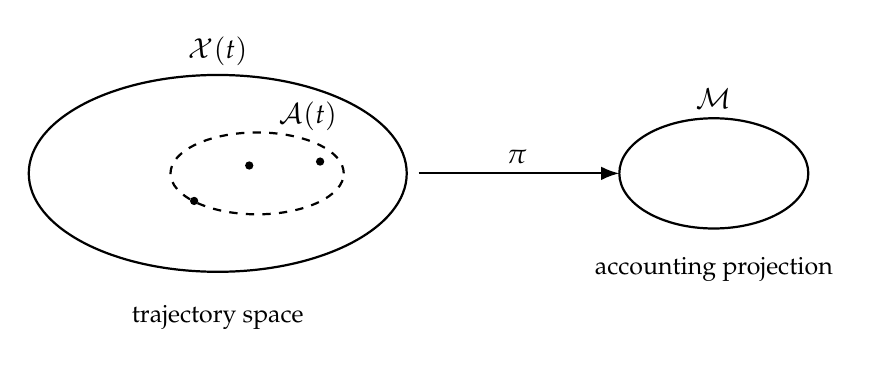
\begin{tikzpicture}[scale=1.0,>=Latex]
  \draw[thick] (-3,0) ellipse (2.4 and 1.25);
  \draw[thick,dashed] (-2.5,0) ellipse (1.1 and 0.52);
  \node at (-3,1.55) {$\Xcal(t)$};
  \node at (-1.85,0.72) {$\Acal(t)$};
  \draw[->,thick] (-0.45,0) -- (2.1,0);
  \node[above] at (0.8,0) {$\pi$};
  \draw[thick] (3.3,0) ellipse (1.2 and 0.7);
  \node at (3.3,0.95) {$\Mcal$};
  \fill (-2.6,0.1) circle (1.5pt);
  \fill (-3.3,-0.35) circle (1.5pt);
  \fill (-1.7,0.15) circle (1.5pt);
  \node[below] at (-3,-1.55) {\small trajectory space};
  \node[below] at (3.3,-0.95) {\small accounting projection};
\end{tikzpicture}
\caption{Projection from ecological trajectory space $\Xcal(t)$ to accounting manifold $\Mcal$. The admissibility manifold $\Acal(t)\subset\Xcal(t)$ (dashed) is the subset compatible with governance assumptions. Proxy permanence failure occurs when $\Acal(t)$ contracts while $\Mcal$ remains fixed.}
\label{fig:projection}
\end{figure}

\begin{figure}[h]
\centering
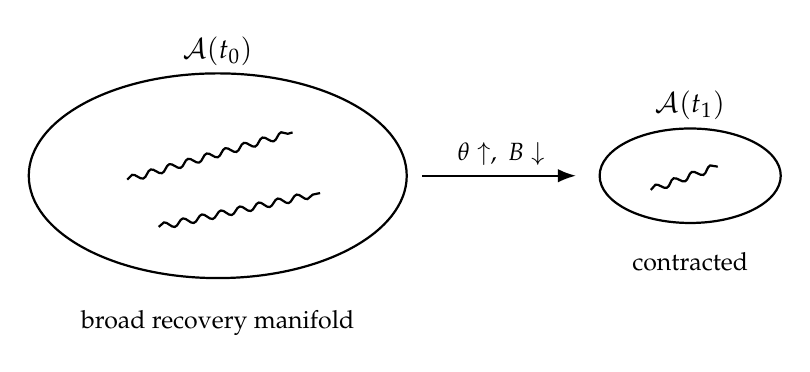
\begin{tikzpicture}[scale=1.0,>=Latex]
  \draw[thick] (-3,0) ellipse (2.4 and 1.3);
  \draw[thick] (3,0) ellipse (1.15 and 0.6);
  \node at (-3,1.58) {$\Acal(t_0)$};
  \node at (3,0.9) {$\Acal(t_1)$};
  \draw[->,thick] (-0.4,0) -- (1.55,0);
  \node[above] at (0.6,0) {\small $\theta\uparrow,\;B\downarrow$};
  \draw[decorate,decoration={snake,amplitude=1.2pt,segment length=7pt},thick]
    (-4.15,-0.05) -- (-2.05,0.55);
  \draw[decorate,decoration={snake,amplitude=1.2pt,segment length=7pt},thick]
    (-3.75,-0.65) -- (-1.7,-0.22);
  \draw[decorate,decoration={snake,amplitude=1.2pt,segment length=7pt},thick]
    (2.5,-0.18) -- (3.35,0.12);
  \node[below] at (-3,-1.58) {\small broad recovery manifold};
  \node[below] at (3,-0.85) {\small contracted};
\end{tikzpicture}
\caption{Admissibility contraction under increasing disturbance forcing $\theta\uparrow$ and biodiversity loss $B\downarrow$. Wavy lines represent accessible recovery trajectories. The manifold shrinks from $\Acal(t_0)$ to $\Acal(t_1)$ while the accounting projection $\Mcal$ remains unchanged.}
\label{fig:contraction}
\end{figure}

\begin{figure}[h]
\centering
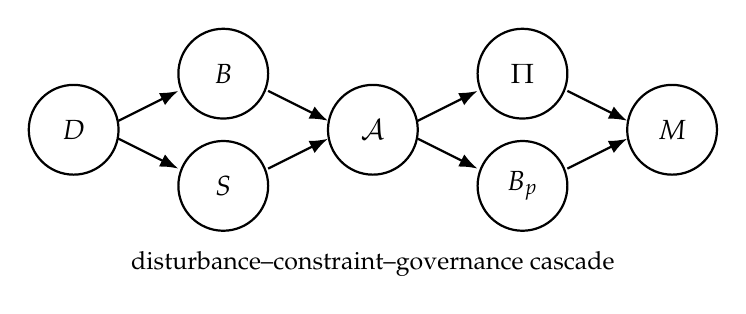
\begin{tikzpicture}[scale=0.95,>=Latex]
  \foreach \x/\lbl in {-4/$D$,-2/$B$,-2.5/$S$,0/$\Acal$,2/$\Pi$,2.5/$B_p$,4/$M$} {
  }
  \draw[thick] (-4,0) circle (0.6);
  \draw[thick] (-2,0.75) circle (0.6);
  \draw[thick] (-2,-0.75) circle (0.6);
  \draw[thick] (0,0) circle (0.6);
  \draw[thick] (2,0.75) circle (0.6);
  \draw[thick] (2,-0.75) circle (0.6);
  \draw[thick] (4,0) circle (0.6);
  \node at (-4,0) {$D$};
  \node at (-2,0.75) {$B$};
  \node at (-2,-0.75) {$S$};
  \node at (0,0) {$\Acal$};
  \node at (2,0.75) {$\Pi$};
  \node at (2,-0.75) {$B_p$};
  \node at (4,0) {$M$};
  \draw[->,thick] (-3.4,0.12) -- (-2.6,0.52);
  \draw[->,thick] (-3.4,-0.12) -- (-2.6,-0.52);
  \draw[->,thick] (-1.4,0.52) -- (-0.6,0.12);
  \draw[->,thick] (-1.4,-0.52) -- (-0.6,-0.12);
  \draw[->,thick] (0.6,0.12) -- (1.4,0.52);
  \draw[->,thick] (0.6,-0.12) -- (1.4,-0.52);
  \draw[->,thick] (2.6,0.52) -- (3.4,0.12);
  \draw[->,thick] (2.6,-0.52) -- (3.4,-0.12);
  \node[below] at (0,-1.5) {\small disturbance--constraint--governance cascade};
\end{tikzpicture}
\caption{Schematic cascade from disturbance pressure $D$ and entropy acceleration $S$, through biodiversity constraint $B$, admissibility $\Acal$, permanence functional $\Pi$, buffer capitalization $B_p$, and market confidence $M$.}
\label{fig:cascade}
\end{figure}

\begin{figure}[h]
\centering
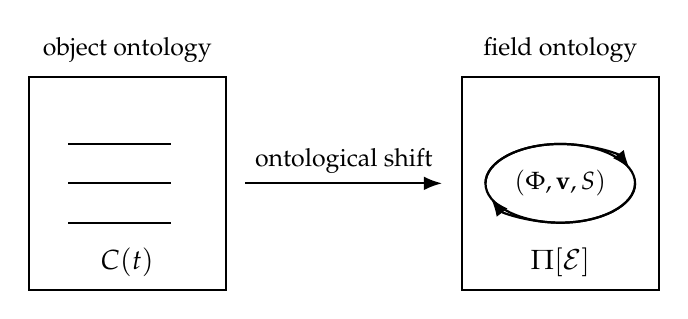
\begin{tikzpicture}[scale=1.0,>=Latex]
  \draw[thick] (-4,-1.35) rectangle (-1.5,1.35);
  \draw[thick] (1.5,-1.35) rectangle (4,1.35);
  \node at (-2.75,1.7) {\small object ontology};
  \node at (2.75,1.7) {\small field ontology};
  \foreach \y in {0.5,0,-0.5}
    \draw[thick] (-3.5,\y) -- (-2.2,\y);
  \node at (-2.75,-1.0) {$C(t)$};
  \draw[thick] (2.75,0) ellipse (0.95 and 0.5);
  \draw[->,thick] (1.8,0) arc(180:22:0.95 and 0.5);
  \draw[->,thick] (3.7,0) arc(0:-158:0.95 and 0.5);
  \node at (2.75,0) {\small $(\Phi,\mathbf{v},S)$};
  \node at (2.75,-1.0) {$\Pi[\Ecal]$};
  \draw[->,thick] (-1.25,0) -- (1.25,0);
  \node[above] at (0,0) {\small ontological shift};
\end{tikzpicture}
\caption{The shift from carbon as a scalar stock $C(t)$ (object ontology, left) to permanence as a field-dependent survival functional over $(\Phi,\mathbf{v},S)$ (field ontology, right).}
\label{fig:ontology}
\end{figure}

\begin{figure}[h]
\centering
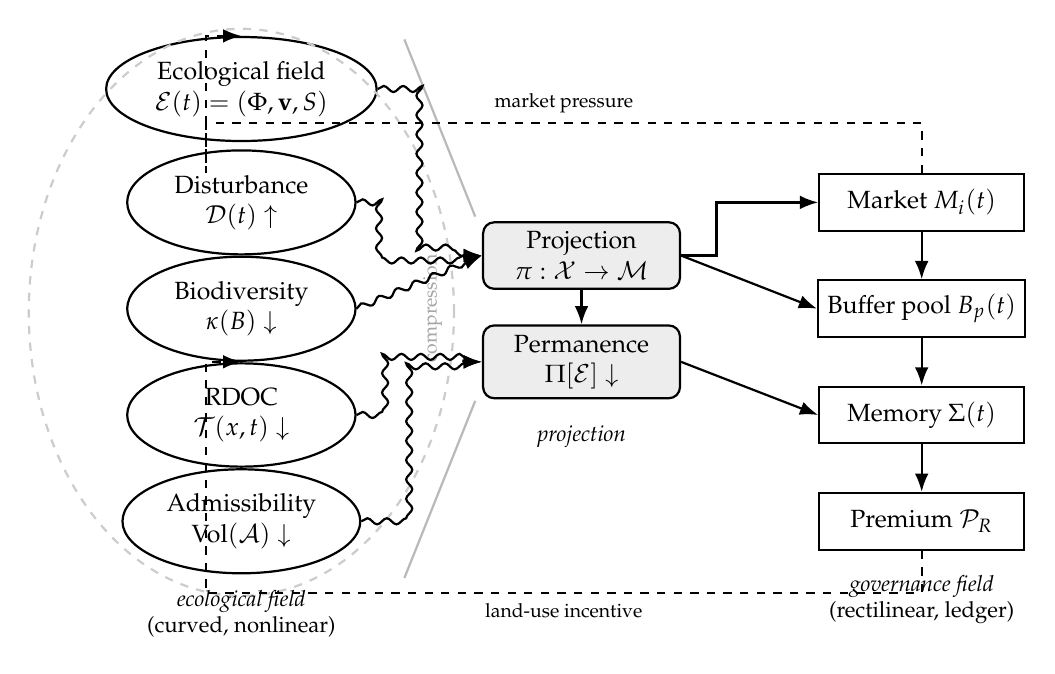
\begin{tikzpicture}[
  scale=0.90,
  >=Latex,
  %% Ecological nodes: ellipses, slightly irregular, field-like
  econode/.style={draw,thick,ellipse,minimum width=2.9cm,minimum height=0.82cm,
                  align=center,font=\small},
  %% Projection nodes: rounded rectangles, intermediate
  projnode/.style={draw,thick,rounded corners=4pt,minimum width=2.5cm,minimum height=0.75cm,
                   align=center,font=\small,fill=black!7},
  %% Governance nodes: strict rectangles, ledger-like
  govnode/.style={draw,thick,rectangle,minimum width=2.6cm,minimum height=0.72cm,
                  align=center,font=\small},
  %% Ecological arrows: wavy, signaling nonlinear dynamics
  ecoarrow/.style={->,thick,decorate,
    decoration={snake,amplitude=1.1pt,segment length=7pt,post length=3pt}},
  %% Governance arrows: straight
  govarrow/.style={->,thick},
  %% Feedback: dashed
  fbarrow/.style={->,thick,dashed}
]

%% ---- ECOLOGICAL FIELD (left) ----
\node[econode] (eco)  at (-4.8, 3.1) {Ecological field\\$\Ecal(t)=(\Phi,\mathbf{v},S)$};
\node[econode] (dist) at (-4.8, 1.5) {Disturbance\\$\mathcal{D}(t)\uparrow$};
\node[econode] (bio)  at (-4.8, 0.0) {Biodiversity\\$\kappa(B)\downarrow$};
\node[econode] (rdoc) at (-4.8,-1.5) {RDOC\\$\Tcal(x,t)\downarrow$};
\node[econode] (acal) at (-4.8,-3.0) {Admissibility\\$\vol(\Acal)\downarrow$};

%% Faint interaction ellipse behind ecology column suggesting nonlinear coupling
\draw[gray!40,thick,dashed,ellipse]
  (-4.8,-0.05) ellipse (3.0cm and 4.0cm);

%% ---- PROJECTION (centre) ----
\node[projnode] (pi)   at (0,  0.75) {Projection\\$\pi:\Xcal\to\Mcal$};
\node[projnode] (perm) at (0, -0.75) {Permanence\\$\Pi[\Ecal]\downarrow$};

%% Funnel lines from ecology to projection boundary
\draw[gray!55,thick] (-2.5, 3.8) -- (-1.5, 1.3);
\draw[gray!55,thick] (-2.5,-3.8) -- (-1.5,-1.3);
\node[font=\scriptsize,gray!70,rotate=90] at (-2.1,0) {compression};

%% ---- GOVERNANCE (right) ----
\node[govnode] (mkt)  at (4.8, 1.5) {Market $M_i(t)$};
\node[govnode] (buf)  at (4.8, 0.0) {Buffer pool $B_p(t)$};
\node[govnode] (mem)  at (4.8,-1.5) {Memory $\Sigma(t)$};
\node[govnode] (prem) at (4.8,-3.0) {Premium $\mathcal{P}_R$};

%% ---- ECOLOGICAL → PROJECTION (wavy) ----
\draw[ecoarrow] (eco.east)  -- ++(0.5,0) |- (pi.west);
\draw[ecoarrow] (dist.east) -- ++(0.35,0) |- (pi.west);
\draw[ecoarrow] (bio.east)  -- (pi.west);
\draw[ecoarrow] (rdoc.east) -- ++(0.35,0) |- (perm.west);
\draw[ecoarrow] (acal.east) -- ++(0.5,0) |- (perm.west);
\draw[govarrow] (pi.south)  -- (perm.north);

%% ---- PROJECTION → GOVERNANCE (straight) ----
\draw[govarrow] (pi.east)   -- ++(0.5,0) |- (mkt.west);
\draw[govarrow] (pi.east)   -- (buf.west);
\draw[govarrow] (perm.east) -- (mem.west);

%% ---- GOVERNANCE INTERNAL (straight, ledger-like) ----
\draw[govarrow] (mkt.south)  -- (buf.north);
\draw[govarrow] (buf.south)  -- (mem.north);
\draw[govarrow] (mem.south)  -- (prem.north);

%% ---- FEEDBACK dashed ----
\draw[fbarrow] (mkt.north) -- ++(0,0.7) -|
  node[near start,above,font=\scriptsize] {market pressure}
  ++(-10.1,-0.7) |- (eco.north);
\draw[fbarrow] (prem.south) -- ++(0,-0.6) -|
  node[near start,below,font=\scriptsize] {land-use incentive}
  ++(-10.1, 0.6) |- (bio.south);

%% ---- COLUMN LABELS ----
\node[font=\footnotesize,align=center] at (-4.8,-4.3)
  {\textit{ecological field}\\(curved, nonlinear)};
\node[font=\footnotesize,align=center] at (0,-1.8)
  {\textit{projection}};
\node[font=\footnotesize,align=center] at (4.8,-4.1)
  {\textit{governance field}\\(rectilinear, ledger)};

\end{tikzpicture}
\caption{Unified causal architecture of the coupled socio-ecological governance system.
\textbf{Left} (ellipses, wavy arrows): the ecological field, rendered with nonlinear
geometry and interacting components suggesting curvature and coupling. The background
ellipse indicates latent nonlinear interactions between ecological variables. \textbf{Centre}
(shaded rounded rectangles): the governance projection $\pi:\Xcal\to\Mcal$ and permanence
functional $\Pi[\Ecal]$; the funnel lines indicate compression of high-dimensional field
structure into a low-dimensional accounting manifold. \textbf{Right} (strict rectangles,
straight arrows): the governance field, rendered rectilinearly to signify ledger logic,
discrete update cycles, and institutional path-dependence. Dashed arrows indicate feedback
from the governance field back into ecological restructuring through market pressure and
land-use incentives. Proxy permanence failure occurs when the centre column becomes
internally coherent within $\Mcal$ while causally decoupled from the left column.}
\label{fig:architecture}
\end{figure}

\section{Principal Notation}
\label{app:notation}

The following table collects the principal variables and operators introduced
across the paper. Readers navigating the notation-dense Sections~8--11 may find it
useful to consult this table alongside the text.

\begingroup
\renewcommand{\arraystretch}{1.3}
\begin{longtable}{@{}p{2.6cm}p{9.6cm}@{}}
\caption{Principal notation.\label{tab:notation}}\\
\toprule
\textbf{Symbol} & \textbf{Meaning} \\
\midrule
\endfirsthead
\multicolumn{2}{l}{\small\itshape Table~\ref{tab:notation} continued}\\
\toprule
\textbf{Symbol} & \textbf{Meaning} \\
\midrule
\endhead
\bottomrule
\endfoot
$\Xcal$ & Full ecological trajectory space \\[2pt]
$\Mcal$ & Low-dimensional accounting projection (governance manifold) \\[2pt]
$\Acal(t)$ & Admissibility manifold: trajectories compatible with governance assumptions at $t$ \\[2pt]
$\Ecal(t)$ & RSVP field triple $(\Phi,\mathbf{v},S)$ \\[2pt]
$\Phi(x,t)$ & Carbon and biomass density \\[2pt]
$\mathbf{v}(x,t)$ & Material-ecological flow (nutrient cycling, DOC export, disturbance propagation) \\[2pt]
$S(x,t)$ & Ecological entropy: $\log\mu(\Omega_x(t))$, log-volume of accessible ecological futures \\[2pt]
$\Tcal(x,t)$ & Transformation accessibility: $\mu(\Omega_x^\text{transform}(t))$, measure of available degradation operators \\[2pt]
$B$ & Biodiversity (species richness or functional diversity) \\[2pt]
$\kappa(B)$ & Constraint-density field: biodiversity-mediated entropy-damping coefficient; $\kappa'>0$ \\[2pt]
$\mathcal{D}(t)$ & Volume of the accessible disturbance manifold at time $t$ \\[2pt]
$\Pi[\Ecal]$ & Permanence functional: $\exp(-\int_0^T\!\Lambda\,d\tau)=\mathbb{P}(\tau>T)$ \\[2pt]
$\Lambda(\tau)$ & Instantaneous destabilization rate: four-term sum over $\mathcal{D}$, $\kappa(B)$, $dS/dt$, $d\ln\Tcal/dt$ \\[2pt]
$\tau$ & First-passage time: $\inf\{t\geq 0:\Phi_t<\Phi_\text{min}\}$ \\[2pt]
$\mathcal{R}(t)$ & Resilience ratio: $\beta\kappa(B)/\alpha\dot{\mathcal{D}}$; phase boundary at $\mathcal{R}=1$ \\[2pt]
$\dim_C$ & Constraint dimensionality: effective number of independent constraint channels \\[2pt]
$\Gcal(t)$ & Governance state vector $(B_p,R_m,L_c,\Sigma)$ \\[2pt]
$B_p,\,R_m,\,L_c$ & Buffer pool capitalization, market confidence, land-use compliance pressure \\[2pt]
$\Sigma(t)$ & Institutional memory: $\int_{-\infty}^t K(t-s)\mathcal{O}(s)\,ds$; decays on timescale $\tau_\text{inst}$ \\[2pt]
$\tau_c$ & Critical governance latency: $\sup\{\tau:\vol(\Acal(t))>0\text{ under update period }\tau\}$ \\[2pt]
$\mathcal{P}_R(t)$ & Resilience premium operator \\[2pt]
$\Xi_D$ & Disturbance entropy pressure: $-\partial_t\log\vol(\Acal_D)$ \\[2pt]
$\Xi_B$ & Constraint-channel erosion rate: $-\partial_t\dim_C$ \\[2pt]
$\Xi_\Sigma$ & Governance entropy: $\|\Sigma(t)-\mathcal{O}(t)\|^2$ \\[2pt]
$\Xi_C$ & Contagion coupling intensity: $\sum_j W_{ij}H(\mathcal{R}_c-\mathcal{R}_j)$ \\[2pt]
$D_\pi$ & Decoupling constant analogue: actual carbon loss / projected buffer pool coverage \\[2pt]
$\alpha,\,\nu$ & RC model parameters: average lifetime of reactive compounds; reactivity distribution shape \\
\end{longtable}
\endgroup

\section{Claim-Status Index}
\label{app:claims}

The following index maps the paper's principal formal objects to their claim status
under the grammar defined in Section~1.

\medskip
\noindent\textbf{[E] Empirical results} (drawn directly from cited papers):
The 6.3$\times$ buffer pool undercapitalization \citep{Wu2026};
the 7--146~PgC biodiversity-driven carbon loss range \citep{Weiskopf2024};
the 14--25\% RDOC fractions and RC model parameters \citep{Watanabe2026};
the $b=0.26$ biodiversity--biomass exponent \citep{OConnor2017};
the voluntary carbon market contraction from \$2.1B to \$700M.

\medskip
\noindent\textbf{[F] Formal definitions and theorems}:
Definition of $S(x,t)=\log\mu(\Omega_x(t))$ (Section~2);
Definition of $\Tcal(x,t)$ (Section~7);
Admissibility manifold and proxy permanence failure (Section~2);
Carbon-balance equation (Section~3);
Admissibility volume theorem and Corollary~1 (Section~6);
Permanence functional and first-passage survival interpretation (Section~4);
Propositions~1--3 (Sections~4--5);
Institutional memory kernel (Section~9);
Critical governance latency Proposition~4 (Section~10).

\medskip
\noindent\textbf{[H] Heuristic correspondences}:
All material in Section~8 (decoupling theory and CLIO);
Section~9 (scale vectors and the negligible-but-constitutive pattern);
The identification of $D_\pi\approx 6.3$ with the decoupling constant;
The TARTAN--wave-packet analogy;
The $\kappa(B)$--scale-vector preconditioning analogy.

\medskip
\noindent\textbf{[C] Conjectural extensions}:
Resilience premium $\mathcal{P}_R(t)$ and its four observables (Section~10);
Self-correcting buffer pool dynamics $dB_p/dt$ (Section~10);
Nonlinear contagion model with threshold $\phi$ (Section~10);
Optimal control law $\mathbf{u}^*$ (Section~10);
Variational action $\mathcal{L}^*$ with synchronization term (Section~10).

\bigskip
\noindent\rule{\linewidth}{0.4pt}
\bigskip

\section{Key Derivations}
\label{app:derivations}

\subsection{Permanence Functional from a Hazard Rate}

Let $\tau$ be the first-passage time and define the survival function $\Pi(t)=\mathbb{P}(\tau>t)$.
If $\Lambda(t)$ is the instantaneous destabilization hazard, then
$\Lambda(t) = -d\log\Pi(t)/dt$.
Integrating from $0$ to $T$ with $\Pi(0)=1$ gives
\begin{equation*}
\Pi(T)=\exp\!\left(-\int_0^T\Lambda(\tau)\,d\tau\right).
\end{equation*}
The permanence functional is therefore not an arbitrary exponential discount; it is the
standard survival functional associated with a time-dependent reversal hazard.

\subsection{Buffer Undercapitalization as Hazard Discrepancy}

Let $\Lambda_0$ be the historical (protocol-calibrated) hazard and $\Lambda_i$ the true
nonstationary hazard for project $i$. Then
\begin{equation*}
D_{\pi,i}
=\frac{B_i^{\mathrm{req}}}{B_i^{\mathrm{prot}}}
=\frac{1-\exp[-\int_0^T\Lambda_i(\tau)\,d\tau]}{1-\exp[-\int_0^T\Lambda_0(\tau)\,d\tau]}.
\end{equation*}
When $\Lambda_i > \Lambda_0$ over a substantial portion of the accounting horizon,
$D_{\pi,i}>1$. The empirical finding $D_\pi\approx 6.3$ is a measured discrepancy
between historical-protocol and nonstationary ecological hazard.

\subsection{Biodiversity-Mediated Carbon Loss (First-Order)}

From $\mathrm{Biomass}=aR^b$, proportional biomass retained when species fraction
$p_R$ survives is $p_R^b$. Thus $\Delta C_\text{bio}=C_0(1-p_R^b)$.
For $p_R=1-\varepsilon$:
$(1-\varepsilon)^b = 1-b\varepsilon+O(\varepsilon^2)$,
giving $\Delta C_\text{bio} = C_0 b\varepsilon + O(\varepsilon^2)$.
Biodiversity loss produces a first-order carbon-storage penalty whenever $b>0$.

\subsection{Resilience Ratio from Entropy Balance}

Ignoring spatial-gradient and noise terms in equation~\eqref{eq:entropy-evo},
entropy production is controlled by the balance
$\alpha D(\theta,t) \lessgtr \beta\kappa(B)$.
For accelerating disturbance, replace the static level $D$ with growth rate
$\dot{\mathcal{D}}$ to obtain the dimensionless resilience ratio
$\mathcal{R}(t) = \beta\kappa(B(t))/\alpha\dot{\mathcal{D}}(t)$.
Persistence requires $\mathcal{R}>1$; collapse cascade follows $\mathcal{R}<1$.

\subsection{Admissibility Volume Monotonicity}

$\vol(\Acal) = \int_\Xcal \mathbf{1}_{\Phi\geq\Phi_\text{min}}\mathbf{1}_{S\leq S_\text{max}}\,d\mu(\gamma)$.
Increasing $B$ increases $\kappa(B)$, reducing $\partial S/\partial t$
(from equation~\eqref{eq:entropy-evo}), extending the set satisfying $S\leq S_\text{max}$,
so $\partial\vol(\Acal)/\partial B>0$.
Increasing $D$ simultaneously raises $\partial S/\partial t$ and lowers $\Phi$,
contracting both indicator conditions, so $\partial\vol(\Acal)/\partial D<0$.

\subsection{RDOC Power-Law Persistence (Derived)}

The RC model sets $k(t)=\nu/(\alpha+t)$. Integrating $\mathrm{DOC}'/\mathrm{DOC}=-k(t)$:
$\log(\mathrm{DOC}(t)/\mathrm{DOC}_0) = -\nu\log((\alpha+t)/\alpha)$,
giving $\mathrm{DOC}(t)=\mathrm{DOC}_0(\alpha/(\alpha+t))^\nu$, which matches
equation~\eqref{eq:rc-model}. The persistence fraction at horizon $T$ is
$\Pi_\text{RDOC}=(\alpha/(\alpha+T))^\nu$.

\subsection{Governance Lag Error (First-Order)}

With $K(s)=\tau_\text{inst}^{-1}e^{-s/\tau_\text{inst}}$ and slowly varying $\mathcal{O}$,
expanding $\mathcal{O}(t-s)=\mathcal{O}(t)-s\dot{\mathcal{O}}(t)+O(s^2)$ and integrating
using $\int_0^\infty K(s)s\,ds=\tau_\text{inst}$ gives
$\Sigma(t) = \mathcal{O}(t) - \tau_\text{inst}\dot{\mathcal{O}}(t) + O(\tau_\text{inst}^2)$.
Governance estimation error is $\mathcal{O}(t)-\Sigma(t) = \tau_\text{inst}\dot{\mathcal{O}}(t)+O(\tau_\text{inst}^2)$,
growing with both institutional memory length and ecological rate of change.

\subsection{Low-Pass Resilience Premium}

With $\mathcal{P}_R^*(t)=\mathcal{P}_0\exp(\sum_i\lambda_i\Xi_i(t))$ and relaxation
equation $d\mathcal{P}_R/dt = -\rho(\mathcal{P}_R-\mathcal{P}_R^*)$, the solution is
$\mathcal{P}_R(t) = e^{-\rho t}\mathcal{P}_R(0) + \rho\int_0^t e^{-\rho(t-s)}\mathcal{P}_R^*(s)\,ds$,
an exponentially weighted moving average with timescale $\rho^{-1}$.

\subsection{Toy Permanence Gap (Closed Form)}

For the two-forest toy model of Section~13:
$\log\Pi_H(T)-\log\Pi_L(T) = \lambda_2 T(\kappa_H-\kappa_L)/\kappa_\text{ref} > 0$.
The permanence gap grows linearly in time and is proportional to the biodiversity contrast,
demonstrating that equal initial carbon stock does not imply equal persistence capacity.

\bigskip
\noindent\rule{\linewidth}{0.4pt}
\bigskip

\bibliographystyle{plainnat}

\begin{thebibliography}{99}

\bibitem[Anderegg et al.(2020)]{Anderegg2020}
Anderegg, W.~R.~L. et al.\ Climate-driven risks to the climate mitigation potential of forests. \textit{Science} \textbf{368}, eaaz7005 (2020).

\bibitem[Anderegg et al.(2022)]{Anderegg2022}
Anderegg, W.~R.~L. et al.\ A climate risk analysis of Earth's forests in the 21st century. \textit{Science} \textbf{377}, 1099--1103 (2022).

\bibitem[Badgley(2024)]{Badgley2024}
Badgley, G. Increasingly active wildfire seasons threaten the sustainability of forest-backed carbon offset programs. \textit{Global Change Biology} \textbf{30}, e17599 (2024).

\bibitem[Badgley et al.(2022)]{Badgley2022}
Badgley, G. et al.\ California's forest carbon offsets buffer pool is severely undercapitalized. \textit{Frontiers in Forests and Global Change} \textbf{5}, 930426 (2022).

\bibitem[Bourgain \& Demeter(2015)]{BourgainDemeter2015}
Bourgain, J.\ \& Demeter, C. The proof of the $\ell^2$ decoupling conjecture. \textit{Annals of Mathematics} \textbf{182}, 351--389 (2015).

\bibitem[Campbell(1979)]{Campbell1979}
Campbell, D.~T. Assessing the impact of planned social change. \textit{Evaluation and Program Planning} \textbf{2}, 67--90 (1979).

\bibitem[Cardinale et al.(2012)]{Cardinale2012}
Cardinale, B.~J. et al.\ Biodiversity loss and its impact on humanity. \textit{Nature} \textbf{486}, 59--67 (2012).

\bibitem[Carlson et al.(2024)]{Carlson2024}
Carlson, A.~K., Yoshimura, T.\ \& Kudo, I. Kelp dissolved organic carbon release is seasonal and annually enhanced during senescence. \textit{Journal of Phycology} \textbf{60}, 980--1000 (2024).

\bibitem[Duffy et al.(2017)]{Duffy2017}
Duffy, J.~E., Godwin, C.~M.\ \& Cardinale, B.~J. Biodiversity effects in the wild are common and as strong as key drivers of productivity. \textit{Nature} \textbf{549}, 261--264 (2017).

\bibitem[Ferrier et al.(2016)]{Ferrier2016}
Ferrier, S. et al.\ \textit{The Methodological Assessment Report on Scenarios and Models of Biodiversity and Ecosystem Services}. IPBES (2016).

\bibitem[Goodhart(1975)]{Goodhart1975}
Goodhart, C.~A.~E. Problems of monetary management: the U.K.\ experience. In \textit{Papers in Monetary Economics} (Reserve Bank of Australia, 1975).

\bibitem[Guth(2016)]{Guth2016}
Guth, L. A restriction estimate using polynomial partitioning. \textit{Journal of the American Mathematical Society} \textbf{29}, 371--413 (2016).

\bibitem[Guth, Maldague \& Oh(2024)]{GuthMaldagueOh2024}
Guth, L., Maldague, D.\ \& Oh, C. $\ell^2$ decoupling theorem for surfaces in $\mathbb{R}^3$. arXiv:2403.18431 (2024).

\bibitem[Guth, Maldague \& Wang(2022)]{GuthMaldagueWang2022}
Guth, L., Maldague, D.\ \& Wang, H. Improved decoupling for the parabola. \textit{Journal of the European Mathematical Society} \textbf{24}, 3205--3222 (2022).

\bibitem[Hansell(2013)]{Hansell2013}
Hansell, D.~A. Recalcitrant dissolved organic carbon fractions. \textit{Annual Review of Marine Science} \textbf{5}, 421--445 (2013).

\bibitem[Haya et al.(2023)]{Haya2023}
Haya, B.~K. et al.\ Comprehensive review of carbon quantification by improved forest management offset protocols. \textit{Frontiers in Forests and Global Change} \textbf{6}, 958879 (2023).

\bibitem[Holland(1992)]{Holland1992}
Holland, J.~H. \textit{Adaptation in Natural and Artificial Systems}. MIT Press (1992).

\bibitem[Hooper et al.(2005)]{Hooper2005}
Hooper, D.~U. et al.\ Effects of biodiversity on ecosystem functioning: a consensus of current knowledge. \textit{Ecological Monographs} \textbf{75}, 3--35 (2005).

\bibitem[Isbell et al.(2015)]{Isbell2015}
Isbell, F., Tilman, D., Polasky, S.\ \& Loreau, M. The biodiversity-dependent ecosystem service debt. \textit{Ecology Letters} \textbf{18}, 119--134 (2015).

\bibitem[Juarrero(1999)]{Juarrero1999}
Juarrero, A. \textit{Dynamics in Action: Intentional Behavior as a Complex System}. MIT Press (1999).

\bibitem[Koehler et al.(2012)]{Koehler2012}
Koehler, B. et al.\ Reactivity continuum of dissolved organic carbon decomposition in lake water. \textit{Journal of Geophysical Research: Biogeosciences} \textbf{117}, G01024 (2012).

\bibitem[Krause-Jensen \& Duarte(2016)]{KrauseJensen2016}
Krause-Jensen, D.\ \& Duarte, C.~M. Substantial role of macroalgae in marine carbon sequestration. \textit{Nature Geoscience} \textbf{9}, 737--742 (2016).

\bibitem[Levin(1998)]{Levin1998}
Levin, S.~A. Ecosystems and the biosphere as complex adaptive systems. \textit{Ecosystems} \textbf{1}, 431--436 (1998).

\bibitem[Loreau \& Hector(2001)]{Loreau2001}
Loreau, M.\ \& Hector, A. Partitioning selection and complementarity in biodiversity experiments. \textit{Nature} \textbf{412}, 72--76 (2001).

\bibitem[Mori et al.(2021)]{Mori2021}
Mori, A.~S. et al.\ Biodiversity--productivity relationships are key to nature-based climate solutions. \textit{Nature Climate Change} \textbf{11}, 543--550 (2021).

\bibitem[Mostovaya et al.(2017)]{Mostovaya2017}
Mostovaya, A. et al.\ Emergence of the reactivity continuum of organic matter from kinetics of a multitude of individual molecular constituents. \textit{Environmental Science \& Technology} \textbf{51}, 11571--11579 (2017).

\bibitem[O'Connor et al.(2017)]{OConnor2017}
O'Connor, M.~I. et al.\ A general biodiversity--function relationship is mediated by trophic level. \textit{Oikos} \textbf{126}, 18--31 (2017).

\bibitem[Odum(1969)]{Odum1969}
Odum, H.~T. The strategy of ecosystem development. \textit{Science} \textbf{164}, 262--270 (1969).

\bibitem[Prigogine \& Stengers(1984)]{Prigogine1984}
Prigogine, I.\ \& Stengers, I. \textit{Order Out of Chaos}. Bantam Books (1984).

\bibitem[Reich et al.(2012)]{Reich2012}
Reich, P.~B. et al.\ Impacts of biodiversity loss escalate through time as redundancy fades. \textit{Science} \textbf{336}, 589--592 (2012).

\bibitem[Rockstr\"{o}m et al.(2021)]{Rockstrom2021}
Rockstr\"{o}m, J. et al.\ We need biosphere stewardship that protects carbon sinks and builds resilience. \textit{PNAS} \textbf{118}, e2115218118 (2021).

\bibitem[Seddon et al.(2019)]{Seddon2019}
Seddon, N. et al.\ Grounding nature-based climate solutions in sound biodiversity science. \textit{Nature Climate Change} \textbf{9}, 84--87 (2019).

\bibitem[Seidl et al.(2017)]{Seidl2017}
Seidl, R. et al.\ Forest disturbances under climate change. \textit{Nature Climate Change} \textbf{7}, 395--402 (2017).

\bibitem[Simon(1962)]{Simon1962}
Simon, H.~A. The architecture of complexity. \textit{Proceedings of the American Philosophical Society} \textbf{106}, 467--482 (1962).

\bibitem[Tilman et al.(1997)]{Tilman1997}
Tilman, D., Lehman, C.~L.\ \& Thomson, K.~T. Plant diversity and ecosystem productivity. \textit{PNAS} \textbf{94}, 1857--1861 (1997).

\bibitem[Wang et al.(2026)]{Wang2026}
Wang, M., Zhu, S., Fang, Y., Li, B., Shen, K.\ \& Zhong, S.
Negligible in size, significant in effect: On scale vectors in large language models.
arXiv:2605.26895 (2026).

\bibitem[Wang \& Loreau(2016)]{Wang2016}
Wang, S.\ \& Loreau, M. Biodiversity and ecosystem stability across scales in metacommunities. \textit{Ecology Letters} \textbf{19}, 510--518 (2016).

\bibitem[Watanabe et al.(2026)]{Watanabe2026}
Watanabe, K., Hori, M., Kubo, A., Moki, H.\ \& Kuwae, T. Macroalgal and seagrass species generate variable amounts of recalcitrant dissolved organic carbon in coastal Japan. \textit{Communications Earth \& Environment} \textbf{7}, 456 (2026). \url{https://doi.org/10.1038/s43247-026-03600-1}

\bibitem[Weiskopf et al.(2022)]{Weiskopf2022}
Weiskopf, S.~R. et al.\ A conceptual framework to integrate biodiversity, ecosystem function, and ecosystem service models. \textit{BioScience} \textbf{72}, 1--12 (2022).

\bibitem[Weiskopf et al.(2024)]{Weiskopf2024}
Weiskopf, S.~R. et al.\ Biodiversity loss reduces global terrestrial carbon storage. \textit{Nature Communications} \textbf{15}, 4354 (2024).

\bibitem[Wu et al.(2026)]{Wu2026}
Wu, C. et al.\ Forest carbon protocols underestimate climate-driven carbon loss risks. \textit{Nature} (2026). \url{https://doi.org/10.1038/s41586-026-10571-y}

\end{thebibliography}

\end{document}
